% !TeX spellcheck = en_US
% !TeX encoding = UTF-8
% !TEX program = pdflatex

% VSCODE word wrap: ALT + Z
% COMPILE WITH:
% `latexmk` 
% latexmk -pdf main.tex
% You need pdflatex and biber (in all TeXLive distributions)

\documentclass[11pt]{book} % text width
\usepackage[utf8]{inputenc} % encode text to utf8


% paragraph formatting: https://www.overleaf.com/learn/latex/Paragraph_formatting
\setlength{\parindent}{1em}
\setlength{\parskip}{1em}


% better language support
\usepackage[english]{babel}

% use pdflatex
\usepackage[T1]{fontenc} % font encoding
\usepackage[a4paper, margin=2cm, head=18.0pt]{geometry} % set margins to 1.5 cm
\usepackage{graphicx}% for graphics
\usepackage{float}
\usepackage[onehalfspacing]{setspace}
\usepackage{tocbasic}
\usepackage{booktabs}
\usepackage{multicol}
\usepackage{multirow}
\usepackage[]{scrlayer-scrpage}
\usepackage[titletoc]{appendix}
\usepackage{comment}
\usepackage{csquotes}% quote
\usepackage{url}
\usepackage{xcolor}
\usepackage{algorithm}
\usepackage{algpseudocode}
\usepackage{dirtree} % directory tree
\usepackage{tikz} % for drawing graphs
\usepackage{tocloft} % merge list of algo and listling
% title and section formatting
\usepackage{titlesec}
\usepackage{longtable}

% quotes and bibliography: https://www.overleaf.com/learn/latex/Typesetting_quotations
\usepackage{csquotes}
\usepackage{dirtytalk}

% glossaries
\usepackage{hyperref}
\usepackage[acronym, toc]{glossaries} 

% code 
\usepackage{listings}


\usepackage{hyphenat} % fix "overfull hbox" with slicing words using hyphenation
% customize the header and footer of the document
\usepackage{scrlayer-scrpage}

\DeclareQuoteStyle{english}{\glqq}{\grqq}{\glq}{\grq}

% \usepackage[
%     backend=biber,
%     style=numeric,
%     sorting=none
% ]{biblatex}
\usepackage[backend=biber, style=numeric, defernumbers=true]{biblatex}
% add commands for automatic cite/uncite distinction
\DeclareBibliographyCategory{cited}
\AtEveryCitekey{\addtocategory{cited}{\thefield{entrykey}}}
\addbibresource{biblio.bib} % bibliography
\nocite{*} % all references

\newcommand{\ts}{\textsuperscript} % superscript for 2nd or XIXème

\pagenumbering{roman} % set page numbering of front matter sections

% use acronyms and glossaries
% toc: add glossary to table of contents

\makeglossaries
% byte
\newacronym{msb}{MSB}{Most Significant Bit}
\newacronym{lsb}{LSB}{Least Significant Bit}
% technical terms
\newacronym{vmi}{VMI}{Virtual Machine Introspection}
\newacronym{ssh}{SSH}{Secure Shell}
\newacronym{regex}{REGEX}{regular expressions}
\newacronym{scp}{SCP}{secure copy}
%static analyse
\newacronym{bfd}{BFD}{Byte Frequency Distribution}
%deep learning
\newacronym{lstm}{LSTM}{Long Short-Term Memory}
\newacronym{gru}{GRU}{Gated Recurrent Units}
\newacronym{rnn}{RNN}{Recurrent Neural Networks}
\newacronym{cnn}{CNN}{Convolutional Neural Networks}
\newacronym{rcnn}{RCNN}{Recurrent Convolutional Neural Network}

\newacronym{seq2seq}{Seq2Seq}{Sequence-to-Sequence}
% machine learning
\newacronym{smote}{SMOTE}{Synthetic Minority Over-sampling Technique}
\newacronym{pca}{PCA}{Principal Component Analysis}
\newacronym{t-sne}{t-SNE}{t-Distributed Stochastic Neighbor Embedding}

\newacronym{knn}{KNN}{K-Nearest Neighbors}
\newacronym{svm}{SVM}{Support Vector Machines}
\newacronym{optics}{OPTICS}{Ordering Points To Identify the Clustering Structure}


% glossaries
\newglossaryentry{pointer}
{ 
    name=pointer,
    description={In our study, pointers are characterized as sequences of hexadecimal numbers that reference distinct memory addresses. These sequences can be recognized using the following regular expression: \texttt{"[0-9a-f]\{12\}0\{4\}"}}
}

\newglossaryentry{chunk}
{
    name=chunk,
    description={In our study, chunks are defined as a series of bytes that are allocated in the heap. These structures are allocated using the \texttt{malloc} function and begin everytime by a \textit{malloc header}}
}

\newglossaryentry{block}
{
    name=block,
    description={8 bytes aligned memory sequence}
}

\newglossaryentry{value_node}
{
    name=value node,
    description={In our study, value nodes represent 8-byte blocks of data that are contained within a structure.}
}


% custom commands
% escape char in latex: https://tex.stackexchange.com/questions/34580/escape-character-in-latex
% horizontal spacing: https://tex.stackexchange.com/questions/74353/what-commands-are-there-for-horizontal-spacing/74354
\newcommand{\p}{\texttt{+}} % small unary plus
\newcommand{\doublep}{\texttt{++}} % double small unary plus
\newcommand{\m}{\texttt{-} \space} % small unary minus
\newcommand{\doublem}{\texttt{-}\texttt{-} \space} % double small unary minus

\hyphenation{hy-phen-a-tion} % indicate all 3 permissible hyphenation points

% where to put all images and figures
\graphicspath{{img/}}

% customize the header and footer of the document
\clearpairofpagestyles
\cfoot[\pagemark]{\pagemark}

% ------------------------------ code listing ------------------------------
\lstset{
  basicstyle=\ttfamily\small,
  breaklines=true,
  frame=single,
  language=bash,
  numbers=left,
  numberstyle=\tiny,
  showstringspaces=false,
  tabsize=1,
  captionpos=b,
  xleftmargin=0pt
}

\lstdefinelanguage{json}{
   basicstyle=\normalfont\ttfamily,
   numbers=left,
   numberstyle=\scriptsize,
   stepnumber=1,
   numbersep=8pt,
   showstringspaces=false,
   breaklines=true,
   frame=lines,
   backgroundcolor=\color{white},
   stringstyle=\color{blue},
   keywordstyle=\color{purple},
   commentstyle=\color{gray},
   string=[s]{"}{"},
   comment=[l]{//},
   morecomment=[s]{/*}{*/},
   keywords={true, false, null}
}


% rename listing to code in captions
\renewcommand{\lstlistingname}{Code}



% merge algorithm and listing lists in the table of listings
\makeatletter
\def\ext@algorithm{lol}% algorithm captions will be written to the .lol file
% share the list making commands and redefine the heading
\AtBeginDocument{%
  \let\l@algorithm\l@lstlisting
  \let\c@algorithm\c@lstlisting
  \let\thealgorithm\thelstlisting
  \renewcommand{\lstlistlistingname}{Algorithms and program code}% List of Algorithms -> List of Algorithms and program code
}
\makeatother
% document info
\newcommand{\thetitle}{Structure embeddings for OpenSSH heap dump analysis}
\newcommand{\theauthor}{Lahoche, Clément Claude Martial}

\title{\thetitle}
\author{\theauthor}
\date{\today}



\titleclass{\chapter}{straight} % make chapters act like sections
\titleformat{\chapter}
  {\normalfont\Huge\bfseries}{\thechapter}{1em}{}
\titlespacing*{\chapter}{0pt}{\parskip}{\parskip}

\setcounter{tocdepth}{3} % set depth of table of contents
\setcounter{secnumdepth}{3}  % Numbering depth of sections

% document content
\begin{document}

% !TeX spellcheck = en_US
% !TeX encoding = UTF-8
\begin{titlepage}
    \centering
    \begin{onehalfspace}
    	
		
\includegraphics[width=7cm, height=1.5cm]{uni-logo.png}
		\hspace*{1.0cm}
		\includegraphics*[width=7cm, height=1.5cm]{Logo_INSA.png}\\
		\vspace{1.0cm}
        	{\Large \bfseries Masterarbeits }\\

        	\vspace{2.5cm}

            \begin{doublespace}
            	{\textsf{\Huge{\thetitle}}}
            \end{doublespace}

        	\vspace{2cm}

            {\Large A report by}\\

        	\vspace{1cm}

        	{\bfseries \large{\theauthor} }\\ ORCID id : 0009-0007-7687-5419
			

        	\vfill

        	{\Large
                \textsc{Pr\"ufer} \\
				Prof. Dr. Harald Kosch \\
                Prof. Dr. Michael Granitzer\\
        	}

        	\vspace{1.5cm}

        	\parbox{\linewidth}{\hrule\strut}

            \vfill

			{\large \today}
    \end{onehalfspace}
\end{titlepage}

\newpage

%%%%%%%%%%%%%%%%%%%%%%%%%%%%%%%%%%%%%%%%%%%%%%%%%%%%%%%%%%%%%%%%%%%%%%%%%%%%%%%%%%%%%%%%%

% -- ABSTRACT
\section*{Abstract}
    \paragraph{}In the dynamic landscape of digital technology, the role of cybersecurity as a cornerstone of IT systems has become increasingly prominent. The escalating complexity of cyber threats has brought digital forensics to the forefront, particularly in the examination of heap dumps from main memory. The Secure Shell protocol (SSH), essential for secure communication, serves a dual purpose: it is a line of defense and a potential channel for malicious activities. This research hones in on predicting SSH keys in OpenSSH memory dumps to strengthen security against unauthorized entry and to aid in the creation of advanced security solutions like honeypots.

    \paragraph{}This Master's thesis is a key component of the SmartVMI project, which is focused on improving AI-powered methodologies for detecting attacks and conducting digital forensics. The thesis investigates the development of data embeddings specifically for analyzing OpenSSH heap dumps and identifying SSH keys, striving for efficacy and uniformity across different OpenSSH versions and uses through machine learning and deep learning techniques. It showcases a broad spectrum of embedding methods, including those based on graphs, statistics, and natural language processing, and evaluates their effectiveness and consistency.

    \paragraph{}The research builds upon the foundational work of SSHkex~\cite{sentanoe_sshkex_2022} and SmartKex~\cite{fellicious_smartkex_2022}, enhancing their methods and outcomes and exploring the possibilities of emerging approaches not yet fully explored.

    \paragraph{}Spanning from October 2022 to October 2023, this document narrates the progression of a year-long Master’s thesis research conducted within the PhDTrack program, a collaboration between the University of Passau and INSA Lyon. Supervised by Prof. Dr. Michael Granitzer and Christofer Fellicious from the University of Passau, and Prof. Dr. Pierre-Edouard Portier from INSA Lyon, the thesis offers a thorough examination of the latest advancements in key prediction for OpenSSH memory dumps. It articulates the research inquiries, experimental setups, development of programs, and the results, while also considering potential directions for future research.

% -- Acknowledgements
\section*{Acknowledgements}
    \paragraph{}My heartfelt thanks are extended to Christofer Fellicious, my esteemed supervisor at the University of Passau, for his invaluable mentorship and support throughout my research journey.

    \paragraph{}I am profoundly grateful to my colleague and dear friend, Florian Rascoussier, for his unwavering technical support and moral encouragement. His partnership in various aspects of this thesis has been instrumental to my Master's experience.

    \paragraph{}I would also like to express my sincere appreciation to my supervisor at INSA Lyon, Prof. Pierre-Edouard Portier, and to Prof. Dr. Michael Granitzer at the University of Passau. Their insights and guidance have significantly enriched my research and academic development.

    \paragraph{}A special acknowledgment is due to the individuals who have supported me in this endeavor, notably Lionel Brunie, Director of the Computer Science Department at INSA Lyon, who has enabled the PhDTrack program from the French side, and Harald Kosch, Head of the Chair of Distributed Information Systems at the University of Passau, who has facilitated this program from the German perspective.

    \paragraph{}I am thankful to Elöd Egyed-Zsigmond, PhDTrack coordinator at INSA Lyon, for his assistance with subject selection and administrative matters, and to Natalia Lucari, also a PhDTrack coordinator at INSA Lyon, for her steadfast support and assistance throughout the program. My gratitude also goes to Ophelie Coueffe, the PhDTrack coordinator at the University of Passau, for her aid and support during this academic journey.

    \paragraph{}I am appreciative of all my fellow PhDTrack students for fostering a collaborative and intellectually stimulating environment, and for the rich discussions that have marked our shared journey over the past two years.

    \paragraph{}Finally, I must express my heartfelt thanks to my family, who have been my constant source of love and encouragement throughout the entirety of this Masterarbeit. 

\newpage

% table of content with list of figures & tables
\tableofcontents
\listoffigures
\listoftables
\lstlistoflistings

\newpage

%%%%%%%%%%%%%%%%%%%%%%%%%%%%%%%%%%%%%%%%%%%%%%%%%%%%%%%%%%%%%%%%%%%%%%%%%%%%%%%%%%%%%%%%%
\pagenumbering{arabic} % reset page numbering of main matter sections


\section{Introduction}\label{chap:introduction}

\begin{comment}
Motivate your research and outline the research gap in this chapter. Why is your thesis relevant and what do you address, what has not been addressed before. 

General Requirements to the thesis:

\begin{itemize}
	\item 60 pages of content in this format. Content does not include table of content, lists, appendices etc.
	\item Proper scientific referencing
	\item Introduction and Background should be less than 50\% of the thesis
	\item Images should be readable and in the proper size. 
\end{itemize}
\end{comment}
 

\paragraph*{}Digital forensics is a linchpin in cybersecurity, enabling the extraction of vital evidence from devices like PCs. This evidence is key for detecting malware and tracing intruder activities. Analyzing a device's main memory is a go-to technique in this field. The fusion of machine learning promises to amplify and streamline these analyses.

\paragraph*{}With the rising need for encrypted communication, Secure Shell (\acrshort{ssh}) protocols are now commonplace. However, these security-focused channels can inadvertently shield malicious actions, posing challenges to standard investigative approaches. Cutting-edge research offers solutions. The work in \citetitle*{fellicious_smartkex_2022}~\cite*{fellicious_smartkex_2022} highlights how machine learning can boost the extraction of session keys from OpenSSH memory images. In a complementary vein, \citetitle*{sentanoe_sshkex_2022}~\cite*{sentanoe_sshkex_2022} showcases the power of Virtual Machine Introspection (\acrshort{vmi}) for direct SSH key extraction.

\paragraph*{}Inspired by \citetitle*{fellicious_smartkex_2022}, this thesis zeroes in on a central challenge: data embedding. While previous studies set the stage for key extraction, the data embedding technique, especially windowing, can be optimized. The design of data embeddings is pivotal for machine learning efficacy, especially in nuanced tasks like memory analysis. This research introduces fresh embedding strategies, aiming to refine extraction and unearth deeper memory snapshot patterns. Merging graph embeddings with advanced machine learning, the goal is to craft a sophisticated toolkit for OpenSSH heap dump studies, bridging digital forensics and machine learning.


\section{Research Questions}

Write down and explain your research questions (2-5)

\section{Structure of the Thesis}

Explain the structure of the thesis. 

\section{Example citation \& symbol reference}\label{sec:citation}
For symbols look at.


\section{Example reference}
Example reference: Look at chapter~\ref{chap:introduction}, for sections, look at section~\ref{sec:citation}.

\section{Example image}

\begin{figure}
	\centering
	
\includegraphics[width=0.5\linewidth]{uni-logo}
	\caption{Meaningful caption for this image}
	\label{fig:uniLogo}
\end{figure}

Example figure reference: Look at Figure~\ref{fig:uniLogo} to see an image. It can be \texttt{jpg}, \texttt{png}, or best: \texttt{pdf} (if vector graphic).

\section{Example table}

\begin{table}
	\centering
	\begin{tabular}{lr}
		First column & Number column \\
		\hline
		Accuracy & 0.532 \\
		F1 score & 0.87
	\end{tabular}
	\caption{Meaningful caption for this table}
	\label{tab:result}
\end{table}

Table~\ref{tab:result} shows a simple table\footnote{Check \url{https://en.wikibooks.org/wiki/LaTeX/Tables} on syntax}
\chapter{Related work}\label{chap:related_work}

\paragraph{}The embedding of memory heap dumps for the detection of SSH keys is a niche yet crucial area of research, especially in the context of cybersecurity and digital forensics. This section reviews two seminal papers that have significantly influenced our work: \textit{SSHKex}, which delves into \acrfull{vmi} and memory forensics, and \textit{SmartKex}, which employs machine learning techniques for SSH key detection.

\section{Virtual Machine Introspection and Memory Forensics: SSHKex}

    \paragraph{}\textbf{SSHKex} is an initiative that delves into the intricacies of analyzing encrypted SSH traffic. By harnessing the capabilities of \acrshort{vmi}, Sentanoe and Reiser spearheaded this project to discreetly extract SSH keys and decrypt SSH network communications, ensuring the preservation of evidence \cite{sentanoe_sshkex_2022}.

    \paragraph{}The methodology adopted by \textbf{SSHKex} seamlessly integrates conventional network traffic monitoring with dynamic SSH session key retrieval. A pivotal assumption is the familiarity with the SSH server's implementation, which is vital for the extraction process. Tools such as LibVMI and Volatility, under the VMI umbrella, are employed to provide an unaltered perspective of the guest VM's state, enabling the efficient pinpointing of SSH session keys within a Linux system's primary memory.


    \paragraph{}Outlined below is the \textbf{SSHKex} key extraction procedure:

    \begin{enumerate}
        \item \textbf{Data Structure Insights}: The technique capitalizes on in-depth understanding of the data structures housing the keys. Debugging symbols, tailored to the SSH version on the target, offer crucial offset values, aiding in key material extraction. Key structures encompass \texttt{struct ssh}, \texttt{struct session\_state}, \texttt{struct newkeys}, and \texttt{struct sshenc}, which collectively house details like IP addresses, session statuses, and encryption keys.
        \item \textbf{OpenSSH Function Tracing}: This step involves tracing functions to accurately locate data structures and timely key extraction. Emphasis is on \texttt{kex\_derive\_keys} (for key generation initiation) and \texttt{do\_authentication2} (triggering user authentication).
        \item \textbf{Breakpoint Implementation}: For debugging purposes, software breakpoints are strategically embedded in the program's execution. Using VMI, SSHKex introduces these breakpoints at the starting points of the two pivotal functions mentioned above.
        \item \textbf{Extraction of Keys}: The \texttt{kex\_derive\_keys} function's invocation prompts SSHKex to initially capture the \texttt{ssh struct}'s address. The subsequent call to the \texttt{do\_authentication2} function facilitates the extraction of actual keys, adhering to recognized structures.
        \item \textbf{Key Classification}: OpenSSH designates distinct indices in the \texttt{newkeys} structure for client-to-server and vice versa keys. SSHKex's extraction is based on these specific indices.
        \item \textbf{Managing Multiple Sessions}: OpenSSH handles numerous SSH sessions by initiating child processes. SSHKex broadens its extraction approach to each child process, identifying them via their distinct process IDs.
    \end{enumerate}

    \paragraph{}A standout feature of \textbf{SSHKex} is its commitment to discretion, conservation, and maintaining evidence authenticity. The methodology is crafted to minimize intrusiveness, ensuring no alterations to the scrutinized system. This is paramount in forensic scenarios where evidence sanctity is of utmost importance.


\section{Machine Learning for SSH Key Detection: SmartKex}\label{sec:related_work:smartkex}

    \paragraph{}\textbf{SmartKex} builds upon the foundation of extracting SSH keys from heap memory dumps, aiming to streamline and automate the process. The project stands out by integrating machine learning techniques, enhancing the efficiency and precision of key extraction. This contrasts with the more complex SSHKex approach, which necessitates in-depth SSH knowledge and breakpoint injections.

    \paragraph{}\textbf{SmartKex} proposes two key extraction methods:
    \begin{itemize}
        \item \textit{Brute-Force Baseline Method}:  A conventional method that sifts through heap memory to identify potential keys by testing decryption.
        \item \textit{Machine Learning-Assisted Method}: Utilizes a Random Forest algorithm, trained on an imbalanced dataset balanced using SMOTE. While this method offers high precision and recall, it's probabilistic, making it less exact than the brute-force approach.
    \end{itemize}

    \subsection{Baseline Brute-Force Method}

    \paragraph{}The brute-force approach of \textbf{SmartKex} encompasses the following steps \cite{fellicious_smartkex_2022}:
    \begin{enumerate}
        \item \textit{Heap Dump Creation}: Binary files of the OpenSSH server process are generated
        \item \textit{Data Trimming}: The method trims irrelevant memory pages based on Hamming distance to reduce heap size.
        \item \textit{Key Search}: The algorithm scans the heap, considering a 128-byte length as a potential key, iterating until the heap's end.
        \item \textit{Decryption Trials}: Each potential key undergoes decryption attempts on network packets. Failed attempts lead to the next potential key.
    \end{enumerate}
    \paragraph{}Despite its exactness, the brute-force method is resource-intensive and is less efficient when keys are towards the heap dump's end.

    \subsection{Machine Learning-Assisted Method}

    \paragraph{}\textbf{SmartKex}'s innovation lies in its machine learning methodology, which, while sacrificing exactness, offers speed and accuracy. The method also reduces the heap to under 2\% of its original size. The steps include:
    \begin{enumerate}
        \item \textit{Heap Dump Inputs}: As with the brute-force method, binary files from OpenSSH are the primary inputs.
        \item \textit{Data Preprocessing}: The heap dump is reshaped into an N × 8 matrix. High entropy sections, potential encryption keys, are flagged using logical operations on byte differences.
        \item \textit{Model Training}: A Random Forest algorithm is trained on 128-byte segments of the processed heap. Given the dataset's imbalance, a stacked classifier approach is employed.
        \item \textit{Key Detection}: Predictions on potential key-containing slices are made using the model, followed by a brute-force extraction.
    \end{enumerate}
    \paragraph{}\textbf{SmartKex} not only outperforms the brute-force method in speed but also excels in accuracy. Its applications span across cybersecurity and memory forensics. The adaptability of its machine learning methodology makes it a valuable asset for both researchers and professionals. The project's open-source nature further enhances its accessibility, with the code available on GitHub.
    

\section{Our Contribution}

\paragraph{}In this research, we delve deep into the realm of SSH key detection by exploring multiple embedding techniques: graph-based, statistical-based, and deep learning-based embeddings. Our approach is twofold. Firstly, we employ these embeddings in conjunction with a classifier model, comparing their performance to determine the most effective method for SSH key extraction from memory heap dumps. Secondly, to address the challenges of consistency across various OpenSSH versions and usages, we implement a clustering approach. This ensures that our embeddings not only accurately detect SSH keys but also maintain coherence and adaptability across different OpenSSH environments.

\section{Background}\label{chap:background}


\paragraph*{}In the complex world of cybersecurity and digital forensics, innovative approaches are crucial for revealing hidden or encrypted information. OpenSSH stands out as a key instrument for ensuring secure communication. The memory snapshots, or heap dumps, of OpenSSH are treasure troves of data. Through graph generation from these dumps, we can uncover the detailed connections between data structures, identified by their malloc headers, and their associated pointers.

\paragraph*{}This research delves deep into the smart embedding of these connections, aiming to use machine learning classifiers to identify structures that contain OpenSSH keys. The journey is not just about representing data through graphs but also about understanding the raw sequences of bytes in the heap dump. Classical techniques like Shannon entropy, \acrfull{bfd}, and bigram frequencies provide foundational knowledge. However, the rapidly evolving domain of deep learning opens up a plethora of avenues. Models such as \acrfull{rnn} \cite{lai_recurrent_2015} (\acrfull{lstm}\cite{hochreiter_long_1997} and \acrfull{gru}\cite{chung_empirical_2014}) and sequence-to-sequence learning \cite{sutskever_sequence_2014} offer unique perspectives on raw byte embedding. Furthermore, the efficacy of convolutional approaches (\acrshort{cnn}), both standalone\cite{lecun_gradient-based_1998} and in conjunction with recurrent networks, for sequence modeling is well-documented \cite{bai_empirical_2018}. Notably, the application of neural networks in file fragment classification, especially with lossless representations, has shown promising results \cite{hiester_file_2018}.Finally, we will dive into transformers\cite{vaswani_attention_2017} and autoencoders.

\paragraph*{}The aim of this background section is to provide a comprehensive overview of graph creation from heap dumps, techniques for raw byte embedding, and their role in identifying OpenSSH key structures. By merging age-old techniques with modern approaches, we strive to highlight the most effective methods for analyzing OpenSSH heap dump.

\subsection{Graph Generation from Heap Dumps}
    \subsubsection{Secure Shell (SSH)}
    
        \paragraph*{}\enquote{The \acrfull{ssh} is designed to enable encrypted communication across potentially unsecured networks, ensuring the confidentiality of data during transmission. Each \acrshort{ssh} session utilizes a specific set of session keys, encompassing six distinct keys:

        \begin{itemize}
            \item \textbf{Key A:} Client-to-server initialization vector (IV)
            \item \textbf{Key B:} Server-to-client initialization vector (IV)
            \item \textbf{Key C:} Client-to-server encryption key (EK)
            \item \textbf{Key D:} Server-to-client encryption key (EK)
            \item \textbf{Key E:} Client-to-server integrity key
            \item \textbf{Key F:} Server-to-client integrity key
        \end{itemize}

        \paragraph*{}To decrypt the encrypted traffic within an \acrshort{ssh} session, knowledge of the IV and EK pair (either Key A with Key C or Key B with Key D) is essential, assuming the presence of passive network monitoring tools. OpenSSH, a prevalent implementation of \acrshort{ssh}, is the primary subject of this research, covering versions from V6\_0P1 to V8\_8P1. OpenSSH incorporates various encryption methodologies, including Advanced Encryption Standard (AES) Cipher Block Chaining (CBC), AES Counter (AES-CTR), and ChaCha20, with IV and EK key lengths varying between 12 and 64 bytes.}
        
        \paragraph*{}This information is derived from the paper titled \citetitle*{fellicious_smartkex_2022} \cite{fellicious_smartkex_2022}.

    \subsubsection{heap dumps of OpenSSH}
        \paragraph*{}\enquote{Heap memory, distinct from local stack memory, is a dynamic memory allocation mechanism. While local stack memory is responsible for storing and deallocating local variables during function calls, heap memory requires explicit memory allocation and deallocation. This is achieved using operators such as \texttt{new} in Java and C++, or \texttt{malloc/calloc} in C.

        \paragraph*{}OpenSSH, which is primarily written in C, employs \texttt{calloc} for memory block allocation. These blocks are designated to store session-related data, including the cryptographic keys. By leveraging this knowledge, one can deduce that if the heap of an active OpenSSH process is dumped at an opportune moment (for instance, during an ongoing SSH session), the resulting heap dump will encompass the \acrshort{ssh} session keys.}

        \paragraph*{}This information is also derived from the paper titled \citetitle*{fellicious_smartkex_2022} \cite{fellicious_smartkex_2022}.

    \subsubsection{Dataset}
        \paragraph{}\enquote{We use SSHKex\cite*{sentanoe_sshkex_2022} as the primary method to extract the \acrshort{ssh} keys from the main memory. In addition, we add two features to SSHKex: automatically dump OpenSSH’s heap and add support for \acrshort{ssh} client monitoring.

        \paragraph{}For this paper, we are using four \acrshort{ssh} scenarios: the client connects to the server and exits immediately, port-forward, secure copy, and \acrshort{ssh} shared connection.
        Two file formats, JSON and RAW, are utilized to store the generated logs. The JSON log file encompasses meta-information, including the encryption name, the virtual memory address of a key, and the key's value in hexadecimal representation (as depicted in Figure~\ref{fig:Background:json}). Conversely, the binary file captures the heap dump of the OpenSSH process (illustrated in Figure~\ref{fig:Background:xxd} using the \texttt{xxd} command).
        \begin{figure}[H]
            \centering
            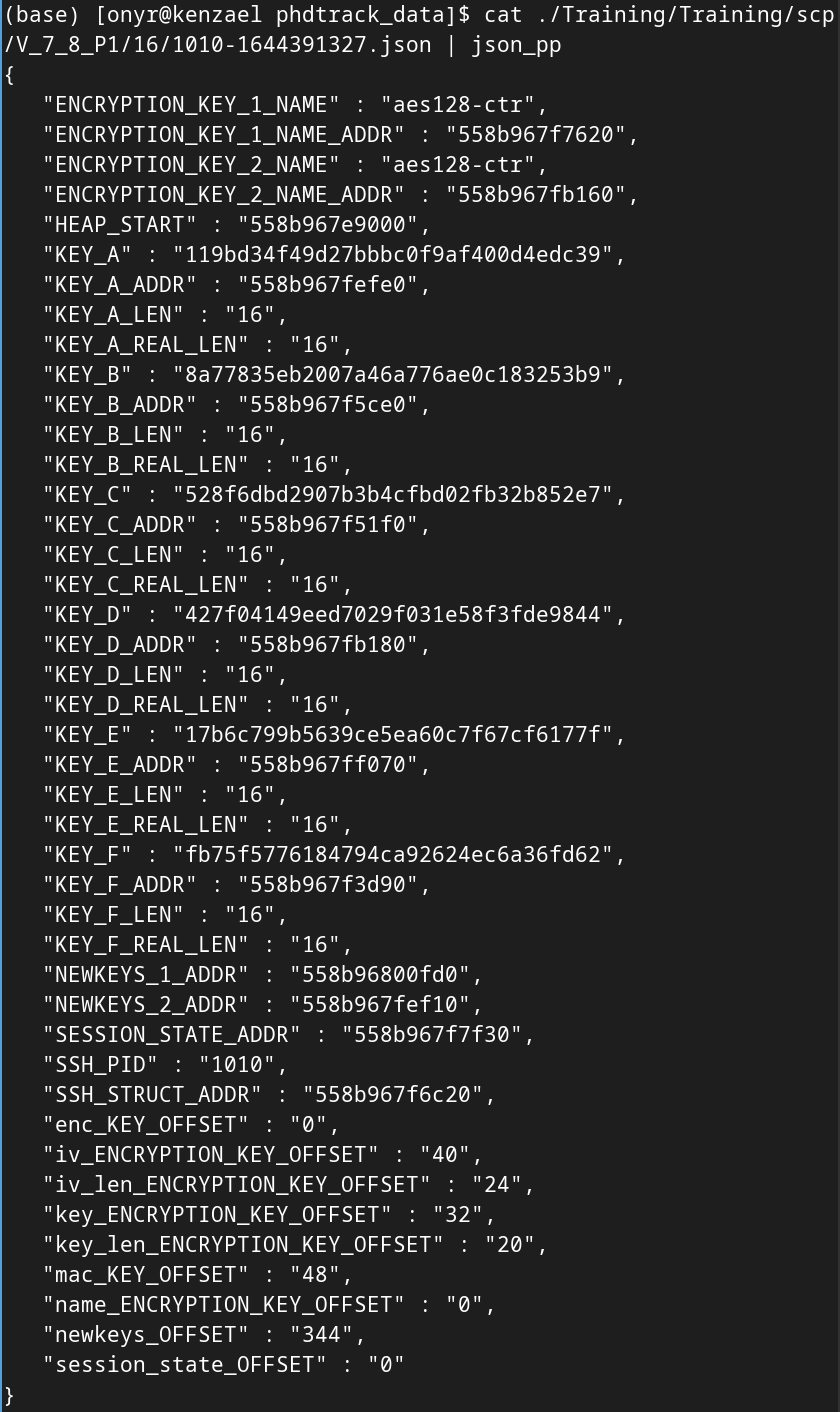
\includegraphics[width=0.6\textwidth]{img/background/json_annotation_for_1010-1644391327.png}
            \caption{Json exemple}
            \label{fig:Background:json}
        \end{figure}

        \begin{figure}[H]
            \centering
            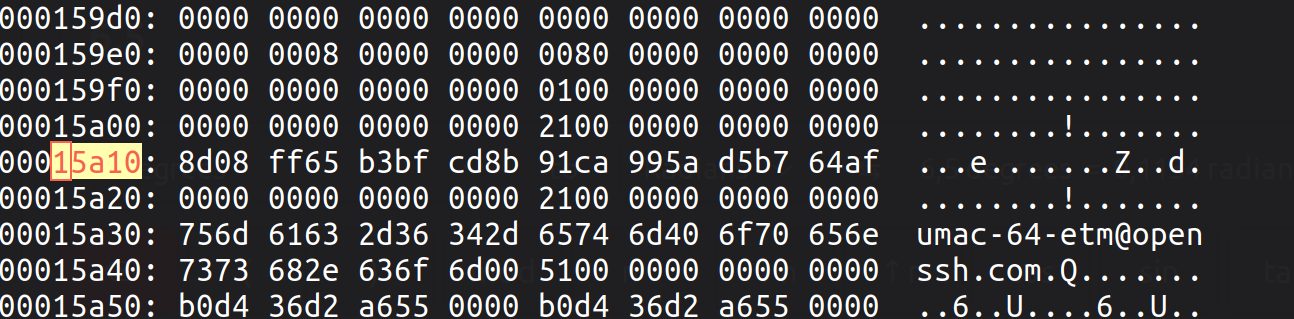
\includegraphics[width=0.6\textwidth]{img/background/xxd.png}
            \caption{Xxd exemple}
            \label{fig:Background:xxd}
        \end{figure}

        \paragraph{}The dataset is structured into two primary directories: \texttt{training} and \texttt{validation}. Each of these directories is further segmented into subdirectories reflecting the specific scenario, such as OpenSSH, port-forwarding, or secure copy (\acrshort{scp}).

        \paragraph{}Subdirectories under OpenSSH or SCP are categorized based on the software version responsible for the memory dump. These directories are further organized by the software version that generated the memory dump. The heaps are then classified based on their key lengths, with each key length possessing its dedicated directory beneath the version directory. These version-specific directories are further divided based on the different key lengths present in a heap.

        \paragraph{}Accompanying every raw memory dump is a JSON file, distinguished by the same alphanumeric sequence, barring the ``-heap'' suffix. This JSON file encapsulates various encryption keys and additional metadata, such as the process ID and the offset of the heap. Consequently, the dataset's utility is not confined to extracting session keys but also extends to identifying crucial data structures harboring sensitive information. The dataset, along with the associated code and tools, is open-sourced. The dataset is accessible via a Zenodo repository\footnote{\url{https://zenodo.org/record/6537904}}. The code can be found in a public GitHub repository\footnote{Link to the GitHub repository}.}
        
        \paragraph{}This data is the same as the data used in the paper titled \citetitle*{fellicious_smartkex_2022} \cite{fellicious_smartkex_2022}.
    
    \subsubsection{Entropy's Role in SSH Key Identification}

        \paragraph{}Encryption keys\cite*{fellicious_smartkex_2022} inherently consist of predominantly random byte sequences. This characteristic stems from the foundational principle of ensuring security through transparency, which guarantees their high entropy. The paper explores the nuances of pinpointing these keys in memory dumps, underscoring the significance of entropy in this endeavor. This particularity can be used to identify the keys in the memory dump.
        
    \subsubsection{Definitions : Structures, Pointers, and the role of malloc headers}
    
        \paragraph{}Through the use of the regular expressions (\acrshort{regex}) \texttt{"[0-9a-f]\{12\}0\{4\}"}, we identified potential \glspl{pointer} within the dump. This heuristic approach acts as a sieve, filtering the extensive data to spotlight possible \gls{pointer} candidates. Nonetheless, it's crucial to understand that while many \glspl{pointer} might be correctly pinpointed, some detected sequences may not be authentic \glspl{pointer}.

        \paragraph{}One notable characteristic of the heap dump is the \textit{malloc header} found at the start of allocated \glspl{structure}. This header, often the initial non-null bytes in a series, signifies the size of the following \gls{structure}. By sequentially reading the heap dump and identifying these headers, it becomes feasible to determine the dimensions and limits of every allocated \gls{structure}, thereby methodically dividing the heap dump into distinct \glspl{structure}.
        
\subsection{Traditional Statistical Embedding}

    \paragraph{}Within the domain of machine learning, how data is represented significantly impacts the performance of models. Even though traditional statistical embedding techniques have been around before many contemporary methods, they continue to be vital in readying data for machine learning endeavors. Rooted in statistical foundations, these techniques provide a methodical approach to transform raw data into concise and meaningful forms. In this subsection, we'll delve into the nuances of entropy and its role in byte sequence embedding, \acrfull{bfd}, and also highlight other classical statistical embedding methods pivotal in data representation for machine learning.
        
    \subsubsection{Entropy and its application in byte sequence embedding}
        \paragraph{}Entropy, a fundamental concept in information theory, quantifies the amount of uncertainty or randomness associated with a set of data. Introduced by Claude Shannon in his groundbreaking work \cite{shannon_mathematical_1948}, entropy serves as a measure of the average information content one can expect to gain from observing a random variable's value.

        \paragraph{}Mathematically, the entropy \(H(X)\) of a discrete random variable \(X\) with possible values \newline \(\{x_1, x_2, \ldots, x_n\}\) and probability mass function \(P(X)\) is given by:
        \begin{align}
            H(X) &= -\sum_{i=1}^{n} P(x_i) \log_2 P(x_i)
            \label{eq:shannon_entropy}
        \end{align}

        \paragraph{}Within the scope of identifying SSH keys, the significance of entropy cannot be understated. Byte sequences exhibiting high entropy typically reflect a multifaceted and varied informational content, traits that are synonymous with encryption keys, especially those in SSH. Sequences with pronounced entropy are often prime contenders for SSH keys due to their inherent randomness and lack of predictability, mirroring the attributes of robust security keys.

        \paragraph{}Fundamentally, entropy acts as a quantitative tool to evaluate the depth of information within data. When applied to SSH, it suggests that data sequences with elevated entropy levels have a heightened probability of correlating with secure keys. This positions entropy as an essential instrument for pinpointing and authenticating SSH keys.
    \subsubsection{Byte Frequency Distribution (BFD)}
        \paragraph{}In the complex world of raw byte embedding, \acrfull{bfd} and n-gram embedding stand out as essential methods, each bringing unique benefits to data representation. \acrshort{bfd} zeroes in on the distribution of individual byte values in a raw byte sequence. Analyzing these distributions allows for the identification of patterns that reflect the inherent nature of the data. This embedding technique becomes particularly relevant when assessing the randomness or structure of byte sequences, such as when detecting encrypted data or pinpointing specific file signatures.

        \paragraph{}On the other hand, n-gram embedding dives deeper into raw byte sequences. Instead of focusing solely on individual bytes, it captures patterns formed by sequences of 'n' consecutive bytes. This approach garners a wider range of contextual information from the raw byte data. For example, a trigram (3-gram) examines patterns formed by three sequential bytes, providing a richer representation than single byte values. Yet, a challenge with n-gram embedding is the potential for the output vector size to grow exponentially as 'n' increases, posing computational and storage issues, especially in real-time scenarios.
        
        \paragraph{}In the realm of raw byte embedding, both \acrshort{bfd} and n-gram techniques offer invaluable perspectives. While \acrshort{bfd} establishes a base representation centered on individual byte frequencies, n-gram embedding enhances it by spotlighting the complex relationships and patterns among consecutive bytes. Together, they form a robust arsenal for representing and analyzing raw byte data in a variety of applications.
    \subsubsection{Other traditional statistical embedding techniques}
        \paragraph{Mean Byte Value}The Mean Byte Value represents the average value of all bytes in a given sequence. It provides an insight into the central tendency of the byte values in the sequence. Mathematically, for a byte sequence \( B \) of length \( n \):
        \begin{equation}
        \text{Mean Byte Value} = \frac{1}{n} \sum_{i=1}^{n} B_i
        \label{eq:mean_byte_value}
        \end{equation}

        \paragraph{Mean Absolute Deviation (MAD)}MAD measures the average distance of each byte value from the mean, providing a sense of the dispersion or spread of the byte values around the mean. It is given by:
        \begin{equation}
        \text{MAD} = \frac{1}{n} \sum_{i=1}^{n} |B_i - \text{Mean Byte Value}|
        \label{eq:mad}
        \end{equation}

        \paragraph{Standard Deviation}Standard Deviation quantifies the amount of variation or dispersion in the byte sequence. A higher value indicates greater variability in the byte values. It is defined as:
        \begin{equation}
        \text{Standard Deviation} = \sqrt{\frac{1}{n} \sum_{i=1}^{n} (B_i - \text{Mean Byte Value})^2}
        \label{eq:standard_deviation}
        \end{equation}

        \paragraph{Skewness}Skewness\cite{wheeler_problems_2011} measures the asymmetry of the distribution of byte values around the mean. A positive value indicates a distribution that is skewed to the right, while a negative value indicates a distribution skewed to the left. It provides insights into the shape of the distribution of byte values. The Fisher’s skewness\cite{cain_univariate_2017} is :
        \begin{equation}
        \text{Skewness} = \frac{n}{(n-1)(n-2)} \sum_{i=1}^{n} \left( \frac{B_i - \text{Mean Byte Value}}{\text{Standard Deviation}} \right)^3
        \label{eq:skewness}
        \end{equation}

        \paragraph{Kurtosis}Kurtosis\cite{wheeler_problems_2011} measures the "tailedness" of the distribution of byte values. A higher kurtosis value indicates a distribution with heavier tails, while a lower value indicates lighter tails. It provides insights into the extremities of the distribution. The Fisher’s kurtosis\cite{cain_univariate_2017} is :
        \begin{equation}
        \text{Kurtosis} = \frac{n(n+1)}{(n-1)(n-2)(n-3)} \sum_{i=1}^{n} \left( \frac{B_i - \text{Mean Byte Value}}{\text{Standard Deviation}} \right)^4 - \frac{3(n-1)^2}{(n-2)(n-3)}
        \label{eq:kurtosis}
        \end{equation}

        \paragraph{n-gram on Bits}When applying n-gram techniques to bits instead of bytes, we focus on sequences of 'n' consecutive bits. For example, a 2-gram on bits would consider patterns formed by two consecutive bits, resulting in four possible combinations: 00, 01, 10, and 11. This approach significantly reduces the size of the output vector compared to byte-based n-grams. By focusing on bits, we can capture more granular patterns in the data while benefiting from a more compact representation, which is computationally efficient and requires less storage.

\subsection{Deep Learning Models for Raw Byte Embedding}

    \paragraph{}In the area of data representation, deep learning is great for understanding raw byte sequences. Just like these models are good at understanding text, they're also good at understanding raw bytes. They can learn and show sequences on their own, which is really helpful for both text and raw bytes. In this section, we'll look at different deep learning models and how they work with raw byte embedding.

    \paragraph{}We'll start with \acrfull{rnn}. Just like they're good with word sequences in text, \acrfull{rnn} are also good with raw byte sequences. Then, we'll look at \acrfull{cnn}, which can find patterns in raw bytes, just like they find patterns in text. After that, we'll talk about Autoencoders, which can learn in a special way. To finish this section, we'll discuss Transformers. They're good at understanding data over a long time, similar to how they understand text.

    \subsubsection{RNNs : Understanding sequence data}
        \paragraph{}\acrfull{rnn} are great tools for text classification. They're good at understanding the deeper meanings in text. Unlike older models that use hand-made features, \acrshort{rnn} can learn and show sequences on their own. This makes them really useful for tasks that deal with sequences. When we think about embedding raw bytes, \acrshort{rnn}'s skill in understanding sequences is similar to how they handle word sequences in text. Here is a list of different \acrshort{rnn} models and their advantages and disadvantages.

        \paragraph{\acrfull{rcnn} for Text Classification\cite{lai_recurrent_2015}:} The \acrshort{rcnn} model, as discussed in the paper by Lai et al., is designed specifically for text classification. Unlike traditional models, \acrshort{rcnn} do not rely on handcrafted features. Instead, they employ a recurrent structure to capture contextual information about words. This approach is believed to introduce considerably less noise compared to traditional window-based neural networks. The model's bidirectional structure ensures that both preceding and succeeding contexts of a word are considered, enhancing its understanding of the word's semantics.

        \begin{itemize}
            \item \textbf{Advantages:} 
            \begin{itemize}
                \item No need for handcrafted features.
                \item Captures richer contextual information.
                \item less noisy.
            \end{itemize}
            \item \textbf{Disadvantages:} 
            \begin{itemize}
                \item Complexity due to bidirectional structure.
                \item Might require more computational resources.
            \end{itemize}; 
        \end{itemize}

        \paragraph{\acrfull{lstm}\cite{hochreiter_long_1997}:}The \acrshort{lstm}, introduced by Hochreiter and Schmidhuber, is a specialized form of \acrshort{rnn} designed to combat the vanishing gradient problem inherent in traditional \acrshort{rnn}. The vanishing gradient problem arises when gradients of the loss function, which are used to update the network's weights, become too small for effective learning. This typically happens in deep networks or when processing long sequences, causing the earlier layers or time steps to receive minimal updates. As a result, traditional \acrshort{rnn} struggle to learn long-term dependencies in the data.

        \paragraph{}\acrshort{lstm} address this issue with their unique cell state and gating mechanisms. The cell state acts as a "conveyor belt" that can carry information across long sequences with minimal changes, ensuring that long-term dependencies are captured. The gating mechanisms, namely the input, forget, and output gates, regulate the flow of information into, out of, and within the cell. This design allows LSTMs to selectively remember or forget information, making them adept at learning and retaining long-term dependencies in sequences.

        \begin{itemize}
            \item \textbf{Advantages:}
            \begin{itemize}
                \item Efficiently learns long-term dependencies; overcomes the vanishing gradient problem inherent in traditional \acrshort{rnn}.
                \item Often achieves faster and more stable learning.
            \end{itemize}
            \item \textbf{Disadvantages:}
            \begin{itemize}
                \item More complex architecture compared to basic \acrshort{rnn} and even \acrshort{gru}.
                \item Can be computationally intensive due to the multiple gating mechanisms.
            \end{itemize}
        \end{itemize}

        \paragraph{\acrfull{gru}\cite{chung_empirical_2014}:} \acrshort{gru} are a variant of \acrshort{rnn} that aim to capture long-term dependencies without the complexity of \acrshort{lstm}. They use a gating mechanism to control the flow of information, making them efficient in sequence modeling tasks.

        \begin{itemize}
            \item \textbf{Advantages:} 
            \begin{itemize}
                \item Simplified structure compared to \acrshort{lstm}.
                \item Efficient in capturing long-term dependencies.
                \item Sometimes outperforms \acrshort{lstm}.
            \end{itemize}
            \item \textbf{Disadvantages:} 
            \begin{itemize}
                \item Still more complex than traditional \acrshort{rnn}.
                \item Might not always outperform \acrshort{lstm} in all tasks.
            \end{itemize}
        \end{itemize}
        

        \paragraph{}To sum it up, \acrshort{rnn} are good at understanding sequences and context. This makes them a good choice for embedding raw bytes. Just like they understand words based on the words around them, \acrshort{rnn} can find patterns in raw byte sequences, giving us a better understanding of the data.
    \subsubsection{CNNs : Pattern detection in raw bytes}
        \paragraph{}\acrfull{cnn}\cite{lecun_gradient-based_1998} are a specialized category of deep learning models adept at identifying patterns. Originally designed for visual data, their prowess extends to tasks like image and document recognition. Drawing inspiration from the human visual cortex's biological processes, \acrshort{cnn} are architected to autonomously and adaptively discern spatial feature hierarchies from inputs. This becomes particularly relevant when considering raw byte embedding, where the goal is to detect patterns in sequences of bytes. The CNN architecture boasts convolutional layers that perform operations on input data to capture localized patterns, and pooling layers that condense spatial dimensions while preserving crucial information. This layered approach enables \acrshort{cnn} to detect intricate patterns by progressively building on simpler foundational patterns. When applied to byte sequences or document recognition, \acrshort{cnn} excel, showcasing remarkable efficacy, especially in tasks like identifying patterns within raw byte sequences or recognizing handwritten content.

        \paragraph{}When tailored to \acrshort{cnn}, the \acrfull{seq2seq}\cite{gehring_convolutional_2017} approach emerges as a potent tool for transforming raw byte sequences into meaningful embeddings. The encoder segment of the \acrshort{seq2seq} model is central to this transformation. It delves into the byte sequence, discerning intricate patterns and nuances, and distills this rich information into a concise context vector or embedding. This condensed representation captures the core essence of the byte sequence, positioning it as a valuable input for subsequent tasks, such as classification models.

        \paragraph{}At the heart of the encoder lie the convolutional layers, skilled in pinpointing specific patterns within the byte sequence. Whether it's unique byte combinations or indicative n-grams, these layers are primed to detect them. As they traverse the raw byte sequence, they employ specialized filters, honed to recognize these specific patterns. As the data flows through the encoder's layers, these identified patterns are synthesized and refined, culminating in a comprehensive embedding of the sequence.

        \paragraph{}Here are two \acrfull{seq2seq} models using \acrshort{cnn} :
        

        \begin{itemize}
            \item \textbf{Autoencoders:} These neural network architectures\cite{hinton_reducing_2006} are designed for data compression and reconstruction. The encoder part compresses the input data into a compact representation, while the decoder reconstructs the original data from this representation. In the context of raw byte sequences, the encoder can be used to generate embeddings that capture the essential patterns and structures of the data.

            \item \textbf{Transformers :} Transformers\cite{vaswani_attention_2017} utilize self-attention mechanisms to weigh the significance of different parts of the input data. This allows them to capture long-range dependencies and relationships in the data. When applied to raw byte sequences, transformers can generate embeddings that consider both local and global patterns, making them particularly effective for tasks that require understanding the broader context of a sequence.

        \end{itemize}
        
        \paragraph{}Yet, a significant challenge with traditional \acrfull{seq2seq} models using \acrshort{cnn} is their constraint in managing inputs of varying sizes. Constructed with a set input size, they face difficulties when presented with sequences of diverse lengths, like raw byte sequences.

        \paragraph{}To address this limitation, various techniques have been employed to normalize the size of the input data. One of the most common methods is \textbf{padding}, where shorter sequences are filled with predefined placeholder values (often zeros) until they match the length of the longest sequence in the dataset. This ensures that all sequences fed into the model have a uniform length. Another approach is \textbf{bucketing}, where sequences of similar lengths are grouped together, minimizing the amount of padding required. Additionally, \textbf{truncation} can be used to shorten sequences that exceed a certain length, although this might result in the loss of some information. While these techniques enable \acrshort{cnn}-based \acrfull{seq2seq} models to handle variable-sized inputs, it's crucial to ensure that the preprocessing steps do not introduce noise or distort the inherent patterns and relationships within the raw byte sequences.
\subsection{Graph Embedding Methods}
    Wait Onyr

\subsection{Machine learning}
    \paragraph{}Machine learning, an integral part of artificial intelligence, revolves around designing algorithms and statistical models that allow computers to perform tasks without being directly programmed. Instead of relying on detailed instructions for every task, machine learning techniques empower systems to learn from data and make data-driven decisions. A key method in this field is supervised learning, in which models are trained using data that comes with predefined labels. Here, each piece of data in the training set has an associated known output. The primary goal of supervised learning is to establish a relationship between inputs and outputs, enabling the model to predict or categorize new, unseen data based on this relationship.

    \paragraph{}A cornerstone in this realm is feature engineering, which involves the meticulous process of selecting and transforming variables to optimize model performance. Another challenge frequently encountered by practitioners is dealing with datasets where some classes are overrepresented, which can skew model predictions. Among the myriad of machine learning models available, certain ones have gained prominence due to their versatility and effectiveness. We will provide an overview of some of these notable models.

\section{Methods}\label{chap:methods}
    \paragraph{}This research dives into the complexities of embedding byte sequences, focusing particularly on the extraction of structures containing SSH keys for machine learning purposes. The varied uses of OpenSSH introduce distinct challenges due to potential variations in the created embeddings. Given the wide array of SSH key dimensions and OpenSSH's intricate operations, maintaining the embeddings' stability and consistency is vital. In this methodological section, we will detail various embedding methods, present a framework for their assessment through a classifier model, and suggest another strategy to verify the embeddings' coherence between the different OpenSSH usage and key sizes.

    
    \subsection{Embeddings}
    \paragraph{}From the Zenodo dataset\ref{seq:background:dataset}, we've isolated distinct memory structures within the raw heap dump files. These structures possess diverse sizes, necessitating the use of an embedding method for classification. Fortunately, a distinguishing feature of each memory structure is the presence of a header, containing vital information such as the structure's size in bytes. To precisely pinpoint the boundaries of each memory structure, we sequentially parse through the raw heap dump files. Beginning the parsing process from the first non-null byte, identified as the header, serves as a marker for the initiation of a new structure. The size data within this header is then leveraged to calculate the exact length of the structure, allowing for the extraction of its entire raw byte data while determining the start of the subsequent one.
    
    \paragraph{}Our next objective centers on the conversion of raw byte data into fixed-size embeddings (\ref{seq:background:traditional_statistical_embedding}, \ref{seq:background:deep_learning_models_for_raw_byte_embedding}), a pivotal step in preparing them for utilization in machine learning applications. Ensuring uniformity in embedding size across all memory structures holds paramount significance. Consistency in embedding dimensions is vital to empower machine learning algorithms for efficient data processing and analysis. This uniformity not only simplifies the integration of memory structures with varying sizes into a coherent classification framework but also acts as a defense against the adverse effects of the curse of dimensionality—a phenomenon that can introduce computational complexities and heighten the risk of overfitting in high-dimensional data spaces. Striking this equilibrium is essential, achieved by maintaining reasonably low embedding dimensions, fostering both efficient data processing and the preservation of essential information within the raw byte data. Additionally, it's worth noting that we will explore various embedding methods to optimize performance.

    \subsection{Embedding quality}
    \paragraph{} Transitioning our focus, we now delve into evaluating the quality of the embeddings. The dataset is notably imbalanced \ref{seq:background:imbalanced_data}, primarily stemming from the rarity of memory structures containing SSH keys, our specific target of interest, within the overall dataset. This rarity results in a significant class imbalance, where the majority of memory structures do not contain SSH keys. To counteract potential bias toward the majority class, we will implement the \acrfull{smote} as a resampling strategy, enabling our model to accurately classify both majority and minority classes. We will then employ a Random Forest model \ref{seq:background:machine_learning}, renowned for its robustness and suitability for high-dimensional data, to carry out the classification task. Our evaluation will rely on metrics such as precision, recall, F1 score, and others to identify the most effective representation for precise classification.

    \subsection{Embedding coherence}
\section{Dataset}
    \paragraph{}The dataset at the core of this thesis, as previously introduced (see \ref{seq:background:dataset}), consists of heap dump raw files related to different OpenSSH use cases and versions. Each heap dump file is paired with a JSON annotation file created by the dataset's creators. These JSON files provide extra information about the heap dump, especially regarding encryption keys. In this section, we will explain our exploration of the dataset, aiming to better comprehend its content and nuances.

    \subsection{Origin}
        \paragraph{}The dataset is derived from heap dumps that capture various OpenSSH usage scenarios. These scenarios encompass four distinct SSH interactions: a straightforward client connection to the server followed by an immediate exit, port-forwarding, secure copying, and SSH shared connection. The heap dumps span different OpenSSH versions and a range of key sizes, from 16 to 64 bytes. These dumps were generated using the SmartKex tool \cite{fellicious_smartkex_2022}. The data collection was conducted on a mini PC equipped with an AMD Ryzen 5500U processor, 16GB of RAM, and a 1TB NVMe SSD, running Debian 11 as its operating system.

    \subsection{Estimating the dataset balancing for key prediction}
        \paragraph{}In this part, our primary objective was to assess the balance of the dataset for key prediction and identify the challenges associated with it.

        \paragraph{}To begin, we aimed to gain an understanding of the dataset's scale. We utilized a code snippet \ref{methods:code:count_all_dataset_files} to count all the files within the dataset, revealing a total of 208,745 files. However, it was imperative to recognize that JSON files, which served as annotation files, were not to be considered part of the raw bytes for embedding. Consequently, these JSON files were excluded from our count to provide a more accurate representation of the dataset's size.

        \begin{lstlisting}[caption={Count all dataset files}, label=methods:code:count_all_dataset_files, language=bash]
        find . -type f | wc -l
        \end{lstlisting}

        \paragraph{}Following this, we employed another code snippet \ref{methods:code:count_raw_files} to specifically count the heap dump raw files, excluding JSON files. This count indicated a total of 103,595 heap dump raw files, which constituted the primary focus of our analysis.

        \begin{lstlisting}[caption={Count heap dump raw dataset files}, label=methods:code:count_raw_files, language=bash]
        find . -type f -name "*.raw" | wc -l
        \end{lstlisting}

        \paragraph*{}To gain further insights into the dataset, we determined its size while excluding annotation files \ref{methods:code:get_dataset_size}. The calculated dataset size amounted to 18,067,001,344 bytes.

        \begin{lstlisting}[caption={Get the size of the dataset}, label=methods:code:get_dataset_size, language=bash]
        find . -type f -name "*.raw" -exec du -b {} + | awk '{s+=$1} END {print s}'
        \end{lstlisting}

        \paragraph{}Considering the nature of the dataset, which featured a maximum of six keys per file, each with a maximum size of 64 bytes, we conducted a rough estimate. We determined that the maximum number of bytes relevant for searching across the dataset was $6 * 64 * 103595 = 39 780 480$ . This calculation accounted for approximately 0.22\% of the dataset's total size.

        \paragraph{}Lastly, it is crucial to acknowledge that the dataset exhibited a significant imbalance and is very large. To address this challenge effectively, strategies were implemented to ensure robust, unbiased analyses, and scalability.
    \subsection*{Annotations}
        \paragraph{}The annotations files are essential to understand the data and how best to utilize them for the study. Each heap dump corresponds to one specific JSON file. To view the contents of these JSON files in a more organized manner, one can reference the method provided at \ref{methods:code:pretty_print_json}. For a clearer understanding, an extract of the JSON annotation from the file located at \path{./Training/client/V_7_8_P1/16/13116-1644920217.json} is available at \ref{methods:code:annotation_extract}.

        \begin{lstlisting}[caption={pretty print JSON}, label=methods:code:pretty_print_json, language=bash]
            python3 -m json.tool file.json
        \end{lstlisting}

        \noindent
        \begin{minipage}{\linewidth}
        \begin{lstlisting}[language=json, caption={An extract of the JSON annotations}, label=methods:code:annotation_extract]
        {
            /* file ./Training/client/V_7_8_P1/16/13116-1644920217.json*/
            "SSH_STRUCT_ADDR": "5619dd7e5570",
            "SESSION_STATE_ADDR": "5619dd7e5df0",
            "KEY_A_ADDR": "5619dd807f40",
            "KEY_A_LEN": "12",
            "KEY_A_REAL_LEN": "12",
            "KEY_A": "34fbe182e76c49a617a93e2e",
            /*...*/
            "KEY_E_ADDR": "5619dd808000",
            "KEY_E_LEN": "0",
            "KEY_E_REAL_LEN": "0",
            "KEY_E": "",
            "KEY_F_ADDR": "5619dd807fd0",
            "KEY_F_LEN": "0",
            "KEY_F_REAL_LEN": "0",
/            "KEY_F": "",
            "HEAP_START": "5619dd7e3000"
        }
        \end{lstlisting}
        \end{minipage}

        \paragraph{}Within these annotation files, several critical pieces of information are present. The ``SSH\_STRUCT\_ADDR'' and ``SESSION\_STATE\_ADDR'' denote the addresses of vital openSSH structures. These addresses are pivotal in gauging the embedding coherence across different openSSH uses and key sizes. If the embeddings of these structures display similarity across various key sizes and openSSH usages, it signifies the embedding's coherence.

        \paragraph{}Other significant annotations such as ``KEY\_A\_ADDR'', ``KEY\_A\_LEN'', ``KEY\_A\_REAL\_LEN'', and ``KEY\_A'' detail the address, length, and value of the key A. In general, six of these annotations can be found for each heap dump. Notably, the ``HEAP\_START'' annotation, along with the length of the heap dump, is of paramount importance. This annotation signifies the starting address of the heap dump. This information not only aids in pinpointing addresses in the heap dump for structures and \glspl{pointer}, but also refines the heuristic used in detecting \glspl{pointer}. By leveraging the ``HEAP\_START'' information, one can verify if a \gls{pointer} is pointing within the heap dump boundaries. As a practical illustration, deducing the address of key A within the heap dump can be achieved by subtracting ``HEAP\_START'' from ``KEY\_A\_ADDR''.

        \paragraph{}However, it's noteworthy that some of these annotation files may be corrupted. Therefore, it's imperative to verify the integrity of each file before its use. In instances where keys are corrupted, such as "KEY\_E" and "KEY\_F" having no recorded values in the extract found at \ref{methods:code:annotation_extract}, it's advised either to remove the corrupted keys or discard the entire file if the data cannot be salvaged.
    
    \subsection{Dataset Validation}
        \paragraph{}The dataset primarily consists of heap dump RAW files, each corresponding to various use cases and versions of OpenSSH. Accompanying each heap dump is a JSON annotation file, crafted by the dataset's creators, to furnish supplementary details, particularly about encryption keys.
        
        \paragraph{}However, the dataset isn't without its flaws. Its application in machine learning has unveiled certain inconsistencies. For example, a few of these files are incomplete, lacking essential data. This poses a challenge since we rely on these annotations to pinpoint key addresses, crucial for annotating memory graphs in the embedding phase. If there's a discrepancy in the format, we'll deem the JSON annotation as corrupted and bypass it. This likely stems from the automated generation of annotations. A case in point is the file in \textit{Training/basic/V\_7\_8\_P1/16/}, which, being the dataset's first file, showcases an incomplete annotation with absent keys. It's vital to be cognizant of these limitations when utilizing the dataset for academic endeavors.
        
        \subsubsection{Annotation Integrity Verification}
            \paragraph{}To accurately gauge the usability of the dataset for machine learning applications, we implemented a validation script named \texttt{check\_annotations.py}. This script is tailored to assess the annotations for their quality, completeness, and consistency.

            \paragraph{}The annotations (JSON files) are categorized as follows:
            \begin{itemize}
                \item \textbf{Complete and Accurate Files}: These files are devoid of missing keys and contain all keys with appropriate values.
                \item \textbf{Malformed Files}: These are files that aren't valid JSON and hence cannot be loaded properly.
                \item \textbf{Inconsistent Files}: Files that present conflicting information within their annotations.
                \item \textbf{Files with Absent Keys}: These files lack certain keys in their annotations. For instance, a JSON file might have "KEY\_E": "", indicating the absence of key E and its corresponding address in the annotation, which poses challenges for accurate machine learning labeling.
                \item \textbf{Files with Incomplete Keys}: These files contain keys but lack the corresponding addresses. An example would be a JSON file with "KEY\_E": "689e549a80ce4be95d8b742e36a229bf", signifying the presence of key E but the absence of its address in the annotation. This again complicates the labeling process for machine learning.
            \end{itemize}

            \paragraph{}The script executes swiftly, processing all the 103,595 JSON annotation files and yields the following outcomes:

            \begin{itemize}
                \item \textbf{Correct and Complete Files}: 26,202 files.
                \item \textbf{Broken Files}: 6 files are identified as broken. Closer inspection reveals these files to be empty.
                \item \textbf{Incorrect Files}: 0 files.
                \item \textbf{Files with Absent Keys}: 58,643 files exhibit missing keys.
                \item \textbf{Files with Incomplete Keys}: 18,750 files display incomplete keys.
            \end{itemize}

            \paragraph{}Delving deeper into the keys:

            \begin{itemize}
                \item \textbf{Total SSH Keys}: 546,534 keys.
                \item \textbf{Missing (Empty) SSH Keys}: 157,244 keys.
                \item \textbf{Incompletely Annotated SSH Keys}: 37,500 keys.
                \item \textbf{Incorrectly Annotated SSH Keys}: 0 keys.
            \end{itemize}

    \subsection{Structure of the Heap File}
        \paragraph{}Heap files serve as the dynamic memory storage for applications, and understanding their structure is crucial for memory analysis. These files are organized in a specific manner, with memory sequences of bytes or "chunks" allocated and deallocated as needed by the application. The heap is 8-byte aligned, which means that we can consider sequences of memory in 8-byte \gls{block}. This alignment ensures efficient memory access and management. To visualize and interpret the heap's structure, tools like memory analyzers or debuggers can be employed.

        \paragraph{}Within the heap, there are four primary types of byte sequences that can be identified with varying degrees of certainty:
        
        \begin{enumerate}
            \item \textbf{Chunk, Malloc Header, and Footer}: We have already discussed these components in detail in an earlier section. In brief, they represent the primary building blocks of the heap, with each chunk being a segment of memory allocated for storing data. The malloc header contains essential metadata about the chunk, and footers, when present, replicate this information.
            \item \textbf{Pointer}: Memory addresses that reference other locations within the heap or other memory segments.
        \end{enumerate}
        
        \paragraph{}Any unidentified user data within these structures is termed as "value data." This data represents the actual content or payload stored within the allocated memory chunks.

        \subsubsection{Chunk}
        \paragraph{}In our exploration of the dataset, the chunk chaining assumption, as detailed in section \ref{seq:background:chunk_chaining}, plays a pivotal role. It's imperative to ensure the integrity of this assumption for accurate analysis. During the dataset refinement process, we identified five heap dumps that contain chunks with a size of 0 bytes, which could potentially violate this assumption. To maintain the reliability of our analyses, these specific dumps have been removed from the dataset. 
        
        \subsubsection{Pointer}\label{seq:methods:dataset:pointer}
            \paragraph{}Pointers are memory addresses that reference other locations within the heap or other segments of memory. In the context of the heap, pointers can indicate data structures, reference other chunks, or provide links in data structures like linked lists or trees. To identify potential pointers within the heap dump, one can utilize the following Reggex :
            \begin{lstlisting}
            1 :/[0-9a-f]\{12}0\{4}
            \end{lstlisting}

            \paragraph{}This command searches for sequences comprising 12 hexadecimal characters succeeded by 4 zeros. The rationale behind this is twofold: 
            \begin{itemize}
                \item The heap dump file's maximum possible addresses typically span around 12 hexadecimal digits.
                \item Pointers' addresses are represented in little-endian format. Consequently, the address's last 4 bytes at 0 are its Most Significant Bytes (MSB).
            \end{itemize}
            \paragraph{}Furthermore, with knowledge of the heap's start addresses and the dump's size, we can enhance the precision of our search. By doing so, we can exclude potential pointers that point outside the boundaries of the dump. Another refinement can be made by verifying if the values pointed to by the potential pointers are 8 bytes aligned, as the heap is structured in 8-byte sequences. However, it's crucial to note that this approach remains heuristic in nature. As such, there's still a possibility of detecting blocks that aren't genuine pointers.
        \subsubsection{Footer}
            \paragraph{}In the GLIBC documentation, the footer of a chunk is expected to mirror the chunk's size as indicated in the malloc header. However, an inconsistency is observed: the size stated in the footer block doesn't always align with this expectation. This deviation is consistently seen across the refined dataset.
    

        

    \subsection{Heap File Distribution}

        
            
        \paragraph{}The dataset offers an in-depth perspective on heap dumps, systematically sorted by key size, OpenSSH version, and distinct use cases. This methodical arrangement streamlines the analytical process, enabling precise investigations tailored to particular criteria. In the subsequent sections, we'll delve into the distribution of the dataset, emphasizing the file count across different use cases, versions, and key sizes, to ensure its suitability for consistent testing.

        
        \subsubsection{Full Dataset}
            \paragraph{}In our initial phase of exploration, we will concentrate on the full dataset. This comprehensive analysis will provide a holistic understanding of the data's structure, variations, and potential anomalies.



            \begin{itemize}
                \item A unique instance was observed where a folder was devoid of any content. This was in the Training section, specifically for the client use case, version V\_7\_8\_P1, and a key size of 64 bytes.
                \item In the Training segment, which comprises 82 combinations of use cases, versions, and key sizes:
                \begin{itemize}
                    \item The minimum number of RAW files present is 923.
                    \item The maximum stretches to 1095. The difference between these two extremes is calculated as:
                    \begin{equation}
                        \frac{\text{max} - \text{min}}{\text{min}} = 0.186
                    \end{equation}
                    This results in a 18.6\% difference.
                \end{itemize}
                \item For the Testing segment, which has 15 combinations:
                \begin{itemize}
                    \item The RAW files range from a minimum of 100 to a maximum of 101, marking a mere 1\% difference between the two.
                \end{itemize}
                \item The Validation segment, with its 82 combinations, shows:
                \begin{itemize}
                    \item A minimum of 151 RAW files.
                    \item A maximum of 211 RAW files. The difference between these values is:
                    \begin{equation}
                        \frac{\text{max} - \text{min}}{\text{min}} = 0.397
                    \end{equation}
                    This presents a 39.7\% difference, yet the number of files remains substantial enough to validate any model effectively.
                \end{itemize}
            \end{itemize}
            
            \paragraph{}The dataset, with its meticulous organization and vast range, offers a robust platform for in-depth analysis and model validation.
            
        \subsubsection{Clean Dataset}
            \paragraph{}Following our examination of the full dataset, we will shift our focus to the cleaned dataset. This refined subset, having undergone meticulous preprocessing and filtering, will offer insights into the most pertinent and reliable data points. Analyzing the cleaned dataset will ensure that our conclusions and subsequent actions are based on high-quality, accurate data.
            
            \begin{itemize}
                \item In the Training segment, which comprises 82 combinations of use cases, versions, and key sizes:
                
                \begin{itemize}
                    \item 63 subdirectories are empty, with no RAW files present.
                    \item The minimum number of RAW files present is 923.
                    \item The maximum stretches to 1079. The difference between these two extremes is calculated as:
                    \begin{equation}
                        \frac{\text{max} - \text{min}}{\text{min}} = 0.169
                    \end{equation}
                    This results in a 16.9\% difference.
                \end{itemize}
                \item For the Testing segment, which had 15 combinations : 0 subdirectories are empty, then no changes are observed.
                \item The Validation segment, with its 82 combinations, shows:
                \begin{itemize}
                    \item 62 subdirectories are empty, with no RAW files present.
                    \item A minimum of 151 RAW files.
                    \item A maximum of 209 RAW files. The difference between these values is:
                    \begin{equation}
                        \frac{\text{max} - \text{min}}{\text{min}} = 0.384
                    \end{equation}
                    This presents a 38.4\% difference, yet the number of files remains substantial enough to validate any model effectively.
                \end{itemize}
            \end{itemize}
            
            \paragraph{}The specifics of the empty folders, including their exact locations and other details, will be cataloged comprehensively in the annex~\ref{sec:annexes:dataset_cleaning_results}. It's crucial to note that due to the invalid nature of the data in these folders, our coherence study on the embeddings will not factor in the OpenSSH version, use case, or key size involved. This decision ensures that our analysis remains rooted in valid and meaningful data, thereby enhancing the reliability of our findings.

            \paragraph{}While the cleaning process did invalidate certain cases within the dataset, it's essential to emphasize that a significant portion remains intact and consequential. These preserved cases provide a robust foundation for our analysis, ensuring that our study is both comprehensive and grounded in meaningful data. The invalidated cases, though notable, do not diminish the overall value and depth of the dataset at our disposal.
    
    \subsection{Keys Analysis}\label{sec:methods:keys_analysis}

        \paragraph{}The analysis of SSH keys within the heap dumps provides crucial insights into their characteristics and behaviors. These findings not only enhance our understanding of the data but also guide subsequent steps in the research process.
    
        \subsubsection{Keys Positions}
    
        \paragraph{}Upon analyzing all the heap dumps, it became evident that all the SSH keys mentioned in the annotations are positioned at the beginning of their respective chunks. These keys have a size ranging from a minimum of 12 bytes to a maximum of 64 bytes. Additionally, the size of the chunks in which these keys are found is consistently observed to be 32, 48, or 64 bytes. This consistent positioning and size uniformity greatly simplify certain embedding processes and offer a streamlined approach to further analysis.

        \subsubsection{Keys Entropy}
    
            \paragraph{}Another significant observation regarding the keys is their high entropy, as referenced in~\ref{sec:related_work:smartkex}. High entropy is indicative of randomness, which is a characteristic feature of cryptographic keys. Leveraging this high entropy~\ref{eq:shannon_entropy} can be instrumental in discriminating the keys from other data. However, it's essential to approach this method with caution. While high entropy can be a strong indicator, it's not foolproof. There's a possibility of encountering false positives, as other high entropy data might exist in the heap. Additionally, there might be instances of false negatives, especially when keys contain multiple repeated bytes by chance.
    
\chapter{Embedding}\label{chap:embedding}

\section{Statistical embedding}
    \paragraph{}Understanding the fundamental concepts of statistical embeddings enables us to delve deeper into the sophisticated processes and practical applications that underscore their significance in embedding tasks. By utilizing statistical techniques, data from high-dimensional spaces is condensed, preserving the inherent probabilistic connections and essential patterns as much as possible.

    \subsection{N-gram values}
        \paragraph{}In reference to section \ref{seq:background:byte_frequency_distribution}, we adopt the use of n-gram values, specifically focusing on the frequency of byte combinations. However, an implication of this approach is that it leads to an exponentially high dimensional space. For instance, with a 2-gram, the potential values amount to $256*256=65536$. Given the extensive dimensionality, we have opted for combinations of bits rather than bytes. This change substantially reduces the space required; a 2-gram, in this case, would only amount to $2*2=4$ values.

        \paragraph{}Switching to bit combinations aligns well with our objectives. Our main interest is in the frequency patterns of n-gram values rather than the specific n-gram values themselves. This is because our core aim is to identify SSH keys, which inherently display frequencies for all combinations due to their random nature.

        \paragraph{}In our approach, we utilize 1-gram, 2-gram, and 3-gram values. As a result, our dimensional space is confined to 14 dimensions, as calculated by $2*2*2+2*2+2=14$. We believe this is an optimal trade-off, striking a balance between the size of the space and the richness of the information it encapsulates.

    \subsection{Other statisticals values}
        \paragraph{}In our approach, several metrics are employed to analyze the data. Specifically, we utilize the mean as detailed in \ref{eq:mean_byte_value}, the standard deviation as found in \ref{eq:standard_deviation}, the MAD from \ref{eq:mad}, the skewness as outlined in \ref{eq:skewness}, the kurtosis referenced in \ref{eq:kurtosis}, and the Shannon entropy from \ref{eq:shannon_entropy}. These metrics, when collectively considered, provide a comprehensive understanding and embed a plethora of information about the data at hand.

        \paragraph{}It's imperative to note a particular aspect of our analysis concerning the standard deviation. There are instances where the standard deviation registers a value of zero. Such an occurrence is indicative of data consistency. Concurrently, in such scenarios, both the kurtosis and skewness are undefined. When faced with this situation, our course of action is to dismiss the \gls{structure} from our analysis. The rationale behind this is straightforward: a consistent \gls{structure} would likely not be pertinent to our exploration, especially when our aim is to identify patterns characteristic of an SSH key, wich are random by nature.
    \subsection{Statistical embedding}
        \paragraph{}We employ then a combination of n-gram values and other statistical metrics to construct the vectors for each \gls{structure}. The n-gram approach contributes 14 distinct values to the vector. Simultaneously, the supplementary statistical metrics, which encapsulate measures of the mean, standard deviation, MAD, skewness, kurtosis, and Shannon entropy, introduce an additional 6 values. Consequently, the resultant vector for each structure comprises a total of 20 values.
    

\section{Graph embedding}\label{sec:embedding:graph_embedding}
    \paragraph{}In this section, we shift our focus towards the creation and embedding of graphs derived from the heap dump data. The process of graph creation involves structuring the data in a way that captures the relationships and connections between the \glspl{structure} and their \glspl{pointer}. Subsequently, we will transform this graphs into low-dimensional vector representations, enabling the application of machine learning techniques to identifying \glspl{structure} containing ssh keys.

    \subsection{Graphs creation}
        \paragraph{}Our graph construction is a meticulously organized process aimed at representing the intricate relationships present within the heap dump data. Comprising three distinct node types - \glspl{structure}, \glspl{pointer}, and \glspl{value_node} - this graph provides a comprehensive view of the data's structure. Our approach commences with the sequential parsing of the heap dump data, enabling the identification of essential \glspl{structure} central to our analytical objectives. These \glspl{structure} form the core nodes of our graph. To establish connections between these \glspl{structure} and their contained data, we further break down each structure into 8-byte blocks. These blocks are then translated into \glspl{value_node} within the graph, serving as connectors bridging the data structures to their specific data. An heuristic approach, grounded in \acrshort{regex}, is employed to identify valid \glspl{pointer} within the heap dump data, with \glspl{pointer} representing a subset of \glspl{value_node}, indicating legitimate \glspl{pointer} references. The scrupulously established connections between \glspl{structure}, \glspl{value_node}, and \glspl{pointer} ensure that the graph accurately mirrors the intricate relationships found within the heap dump data. This comprehensive graph construction process is efficiently implemented in Rust, making effective use of the Petgraph library to handle the complexities of heap dump data and graph representation, offering superior efficiency compared to a Python-based implementation.

        \paragraph{}In the following image \ref{fig:graph_embedding:graph_creation_process}, we can see the \glspl{structure} nodes representing in blue, containing \glspl{pointer} nodes in orange and \glspl{value_node} nodes in gray. 

        \begin{figure}[H]
            \centering
            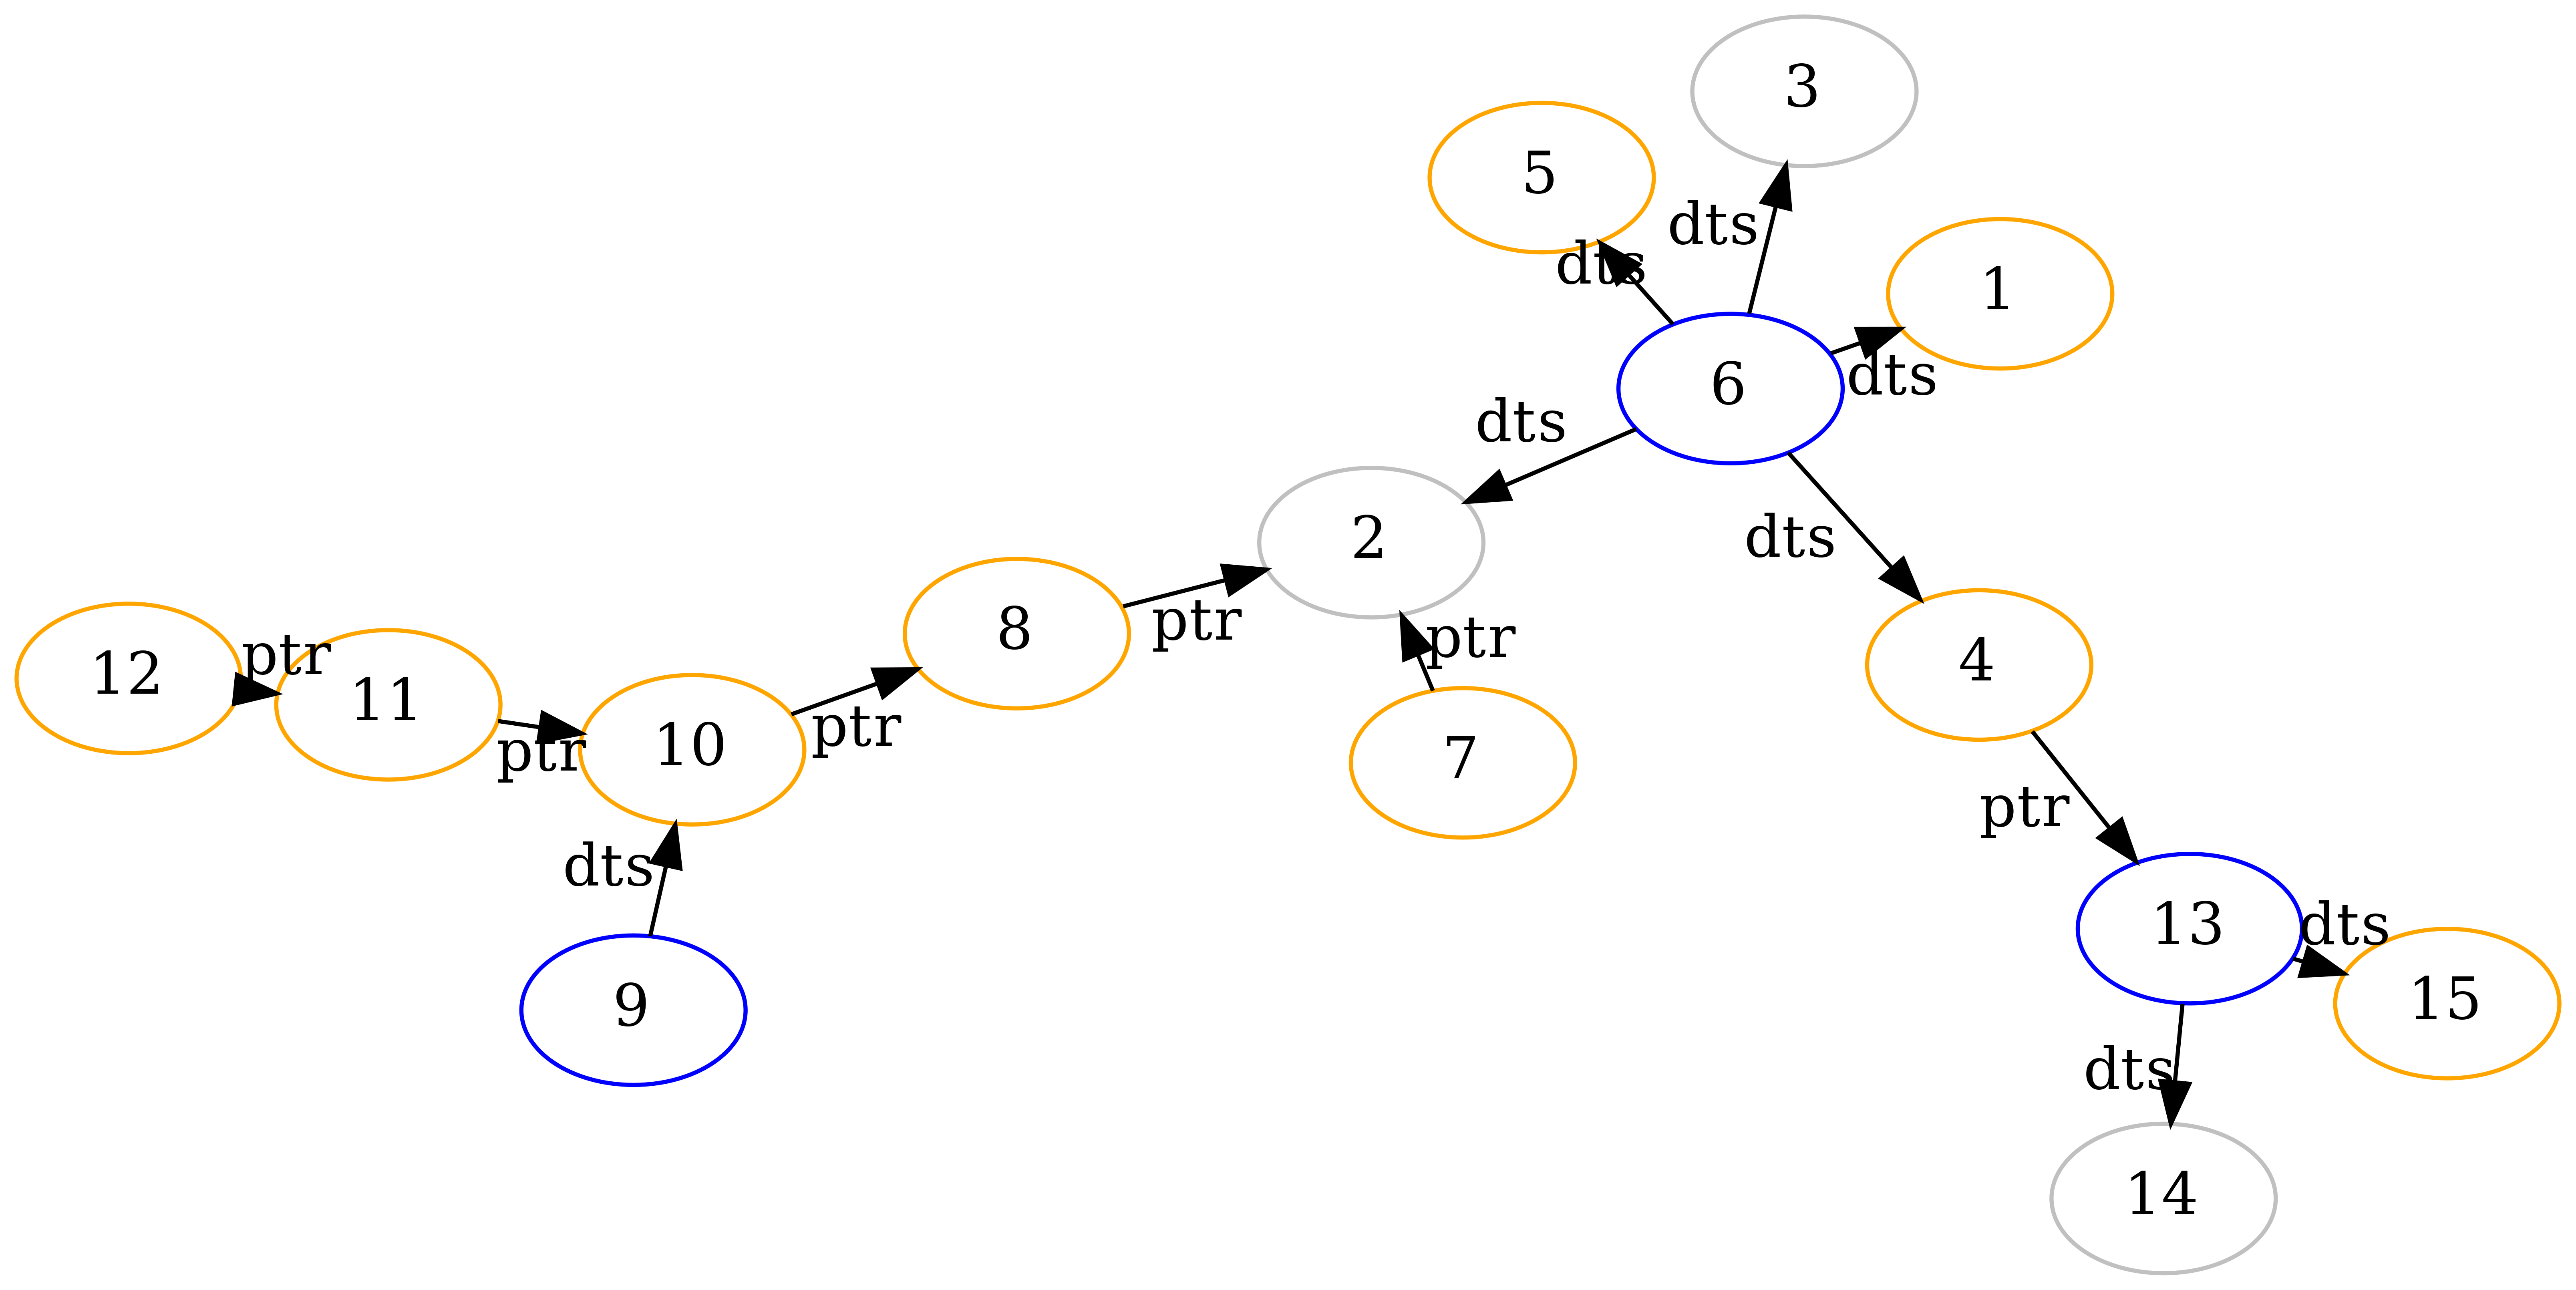
\includegraphics[width=0.9\textwidth]{img/graph_embeding/graph_explain.png}
            \caption{Graph creation process}
            \label{fig:graph_embedding:graph_creation_process}
        \end{figure}

        \paragraph{}After the construction of the graph, we can use graphviz (and the DOT language)\cite{farin_graphviz_2004} to visualize the graph, using the command :
        \begin{lstlisting}[language=bash]
            sfdp -Gsize=67! -Goverlap=prism -Tpng dot_file > image.png
        \end{lstlisting}

        \paragraph{}The following image is an example of the creation of the graph from the file \path{./Training/Training/scp/V_7_8_P1/16/302-1644391327-heap.raw} without \glspl{value_node} to enhance clarity.
        \begin{figure}[H]
            \centering
            \includegraphics[width=0.9\textwidth]{img/graph_embeding/test_graph_from_302-1644391327_no_vn-sfdp.png}
            \caption{Graph example}
            \label{fig:graph_embedding:graph_example}
        \end{figure}

    \subsection{Graphs embedding}

        \paragraph{}Our next step is to uncover deeper insights and semantic understanding from our constructed graph, focusing on semantic embedding. This is the process through which we reshape our graph into a low-dimensional vector space, with each vector acting as a repository for a \gls{structure}'s immediate neighborhood. Through this transformative journey, our aim is to forge vector representations that empower the application of cutting-edge machine learning techniques.

        \paragraph{}To create a concise yet informative representation, considering both structure-to-member and pointer-based connections, we meticulously count the number of \glspl{pointer} and \glspl{structure} directly referencing a specific \gls{structure}'s members. This initial count provides valuable insights into the \gls{structure}'s immediate context. However, we doesn't stop there; we expand this representation by including counts of \glspl{pointer} and \glspl{structure} pointing to those preceding nodes, allowing us to capture deeper layers of context. This recursive process continues until we reach a predetermined depth. Furthermore, we initiate a parallel analysis in reverse, meticulously tracing connections by following \glspl{pointer} from the initial \gls{structure} to capture its children, recursively delving deeper until we reach the specified depth. We can see the algorithm here \ref{algo:embedding:generate_ancestor_children_embedding}. The result is a low-dimensional vector that intricately encodes the \gls{structure}'s neighborhood, offering a comprehensive view of its relationships and contextual significance within the graph.

        \begin{algorithm}[H]
            \caption{Generate Ancestor/Children Embedding}
            \label{algo:embedding:generate_ancestor_children_embedding}
            \begin{algorithmic}
                \Function{GenerateNeighborsDTN}{$structure\_node, dir$}
                    \State $ancestor\_nodes \gets$ an empty set
                    \State $children \gets$ graph.neighbors\_directed($structure\_node, OUT$) \Comment{Get members of the structure}
                    \For{$child$ \textbf{in} $children$}
                        \State $ancestor\_nodes$.insert($child$)
                    \EndFor
                    \State $result \gets$ an empty list
                    \State $current\_nodes \gets$ an empty set
                    \For{$\_$ \textbf{in} $0$ \textbf{to} $DEPTH$}
                        \State $current\_nodes \gets$ $ancestor\_nodes$ \Comment{switch ancestor nodes and current nodes}
                        \State $ancestor\_nodes \gets$ an empty set
                        \State $nb\_dtn \gets 0$
                        \State $nb\_ptr \gets 0$
                        \For{$current\_node$ \textbf{in} $current\_nodes$}
                            \If{$node$ is DataStructureNode} \Comment{Update number of structures and pointers}
                                \State $nb\_dtn \gets nb\_dtn + 1$
                            \ElsIf{$node$ is PointerNode}
                                \State $nb\_ptr \gets nb\_ptr + 1$
                            \EndIf
                            \Comment{Get neighbors of the current node}
                            \For{$neighbor$ \textbf{in} graph.neighbors\_directed($current\_node, dir$)}
                                \State $ancestor\_nodes$.insert($neighbor$) \Comment{Add neighbors to the next ancestor nodes}
                            \EndFor
                        \EndFor
                        \State $result$.append($nb\_dtn$) \Comment{Add number of data structures}
                        \State $result$.append($nb\_ptr$) \Comment{Add number of pointers}
                    \EndFor
                    \State \textbf{return} $result$
                \EndFunction
            \end{algorithmic}
        \end{algorithm}
        
        \paragraph{}We can apply this algorithm to every \gls{structure} within each graph, delving to a depth of 8, which produces an embedding of 32 units: 8 for ancestor \glspl{pointer}, 8 for ancestor \glspl{structure}, 8 for child \glspl{pointer}, and 8 for child \glspl{structure}. To accurately represent the \gls{structure}'s neighborhood, it's crucial not to omit details about its members. Thus, we incorporate the count of \glspl{pointer} in the members and the \gls{structure}'s dimensions. This results in a final embedding size of 34 - 32 for the neighborhood and an additional 2 for the \gls{structure} size and \gls{pointer} count. However, there are inherent challenges with this embedding. It tends to get polluted by the value node, which often lacks significant meaning. Moreover, the relationships between the structures are intricate, and there's potential to represent them in a more straightforward manner.

        
        
\chapter{Embedding quality}\label{chap:embedding_quality}
\section{Embedding Coherence}\label{chap:embedding_coherence}
\paragraph{}A significant facet of this thesis revolves around the comparison of embeddings derived from various use cases, versions, and key sizes of OpenSSH. The objective is to discern whether there exists a coherent relationship among them. To facilitate this comparison, a clustering algorithm is employed to categorize the different embeddings and assess their mutual coherence.

\subsection{Detailed Clustering Approach}
    \paragraph{}For the clustering of embeddings, we opt for the OPTICS algorithm, as referenced in section~\ref{seq:background:optics}. OPTICS is particularly well-suited for this task due to its proficiency in handling data with varying cluster densities, a common characteristic of our embedding data.

    \paragraph{}In our clustering approach, we utilize the cosine distance metric. This choice is strategic, as it mitigates the challenges posed by the curse of dimensionality, eliminating also the need for data scaling prior to clustering. The cosine distance provides a measure of similarity that is not influenced by the magnitude of the data, focusing solely on the direction of the data points in the high-dimensional space.

    \paragraph{}To determine the optimal number of clusters for each embedding, we employ the xi parameter of the OPTICS algorithm. A range of xi values is tested, and the configuration yielding the highest silhouette score is selected. The silhouette score serves as a quantitative measure of the quality of the clustering, with higher values indicating more distinct and well-separated clusters.

    \paragraph{}In our implementation, we resort to the brute force method to compute the cosine metrics, ensuring accuracy in our distance calculations at the expense of computational efficiency. This method systematically calculates the cosine distance between all possible pairs of data points, providing a comprehensive assessment of the similarities and differences among the embeddings

\subsection{Limits and Adaptation}
    \paragraph{}Clustering algorithms, while powerful, come with their own set of challenges, particularly in terms of computational demands. They are known for their high memory consumption and intensive calculations, which can pose constraints when dealing with large datasets. As a result, there's often a need to limit the number of input data points or samples to ensure efficient processing.
    
    \paragraph{}A straightforward, albeit non-optimal, strategy to reduce the number of samples is random sampling. While this approach might not capture the full diversity and nuances of the dataset, it offers a feasible starting point for preliminary analyses. To maintain coherence and representativeness in the sampled data, it's essential to preserve the ratio of significant labels, such as keys and SSH structures (SSH\_STRUCT and SESSION\_STATE), to noise points. This ensures that the key characteristics of the dataset are retained in the sample.
    
    \paragraph{}However, it's worth noting that this sampling method doesn't guarantee that all possible file variations are represented in the sample. Despite its limitations, random sampling serves as an initial approach, providing a snapshot of the dataset's characteristics and offering insights that can guide further, more detailed analyses.
    

\chapter{Results}\label{chap:results}

\paragraph{}In this thesis, we undertake a thorough investigation of data embeddings and their effectiveness in predicting SSH keys within OpenSSH memory dumps. The results are methodically structured, starting with Data Preprocessing, where we lay a solid foundation by preparing the data for in-depth analysis. We proceed to evaluate Deep Learning Models, analyzing their architecture and limitations. This is succeeded by Feature Engineering, where we meticulously refine our data to improve model accuracy. Through Clustering analysis, we explore and identify underlying patterns within the data. Ultimately, we employ Classification techniques to accurately predict and categorize SSH keys, thus demonstrating the practical implications and utility of our research. 
    

\section{Data Preprocessing}

\paragraph{}In the data preprocessing stage, we meticulously calculated each embedding four times, which included the deep learning models. This repetition was to test all combinations of the two filters—entropy and chunk size. The purpose of this thorough approach was to discern the effectiveness of each filter, both individually and in combination, providing us with a clearer understanding of their impact on the data and the subsequent results. The different datasets used are detailed in Section \ref{sec:annexe:all_dataset}. The dataset codes are explained in the following table~\ref{tab:results:dataset_codes}:

\begin{table}[ht]
    \centering
    \begin{tabular}{|p{0.3\linewidth}|p{0.6\linewidth}|}
    \hline
    Dataset Code & Meaning \\ 
    \hline
    value\_node\_embedding & First graph embedding, with all nodes~\ref{sec:embedding:first_graph} \\ \hline
    chunk\_top\_vn\_semantic\_embedding & First graph embedding, keeping only the first block of each chunk~\ref{sec:embedding:first_graph_only_first_block} \\ \hline
    chunk\_semantic\_embedding & Second graph embedding~\ref{sec:embedding:updated_graph} \\ \hline
    chunk\_statistic\_embedding & Statistical embedding~\ref{sec:embedding:statistical} \\ \hline
    chunk\_start\_bytes\_embedding & Start bytes embedding~\ref{sec:embedding:trim_method} \\ \hline
    chunk\_extraction & Raw byte extraction with filters, to be fed into the deep learning model\\ \hline
    \end{tabular}
    \caption{Meanings of Dataset Codes}
    \label{tab:results:dataset_codes}
\end{table}


\section{Deep Learning Models}

\paragraph{}The exploration of hyperparameters is documented in Section \ref{sec:annexes:deep_learning_hyperparameters}. During our experiments, we encountered instances where some models either ran out of memory, as noted in Sections \ref{sec:annexe:out_of_memory_instances_classifications} and \ref{sec:annexe:out_of_memory_instances_clustering}, or experienced timeouts, detailed in Section \ref{sec:annexe:timeout_instances}. Consequently, our discussion will be confined to the results yielded by the models that successfully completed their runs.

\paragraph{}Within the cohort of operational deep learning models, we endeavored to identify the most proficient instance for each algorithm, whether it was Transformers or Word2Vec. However, we encountered a scarcity of successful instances, which impeded our ability to conclusively determine the optimal hyperparameters or to fully understand their impact on the classification metrics. It was observed that instances with a larger word size and a reduced embedding dimension were more likely to succeed, presumably due to the decreased computational load they required.

\section{Feature Engineering}
\paragraph{}During our feature engineering phase, we encountered a challenge that led to the elimination of certain embeddings. This was due to the invariance observed in the columns, an issue that is elaborated upon in Section \ref{sec:annexe:feature_engineering_fails}. The specific embedding that was rendered ineffective and subsequently removed was the semantic embedding of the first graph, as discussed in Section \ref{sec:embedding:graph_embedding}. This elimination was necessary regardless of whether the filter on the first block of each chunk was applied. The primary shortcoming of this embedding was its inability to generate a sufficient number of ancestors to provide useful information. This inadequacy arose because only a minor segment of the value nodes were being pointed to by pointers, which significantly limited the utility of the embedding. In contrast, the second graph managed to compress the information effectively, thereby validating the semantic embedding by conveying more meaningful data for each node.

\paragraph{}The instances that successfully passed the feature engineering stage are meticulously recorded in Section \ref{sec:annexe:feature_engineering_results}. Here, the eight most significant columns are identified.

\section{Clustering}
\paragraph{}In the clustering phase of our analysis, we categorized the data into distinct groups: label 1 for SSH keys, label 2 for "ssh\_struct", label 4 for "session\_state\_struct", and label 0 for the remainder. The detailed outcomes of this clustering are presented in appendix \ref{sec:annexe:clustering_results}. Our examination revealed that the majority of clusters did not exhibit discernible patterns. However, certain datasets, such as those represented by chunk\_start\_bytes\_embedding (23) in Table \ref{tab:23_single_instance_clustering_results} and chunk\_statistic\_embedding (18) in Table \ref{tab:18_single_instance_clustering_results}, maintained a ratio of labels similar to that of the original dataset.


\paragraph{}Interestingly, the clusters derived from deep learning models typically displayed an even distribution of labels, with approximately one quarter of the data falling into each category. An exception to this trend was observed in the Word2Vec 3 Clustering Results on dataset 25 (with chunk size filter), as shown in Table \ref{tab:25_word2vec_3_clustering_results}, which consisted of three clusters with seemingly random label proportions.

\paragraph{}The results from the clustering analysis were not entirely definitive, indicating that there is substantial room for improvement in the methodology. Future efforts in this area would benefit from a more refined approach to enhance the clarity and significance of the clustering outcomes.

\section{Classification}

\paragraph{}The classification results of our study, detailed in appendix \ref{sec:annexe:classification_results}, yielded highly promising results. The performance of various instances, particularly in terms of accuracy, is depicted in the graphical representation found in Figure \ref{fig:results:best_accuracy_instances}, which ranks the instances from best to worst.

\begin{figure}[ht]
    \centering
    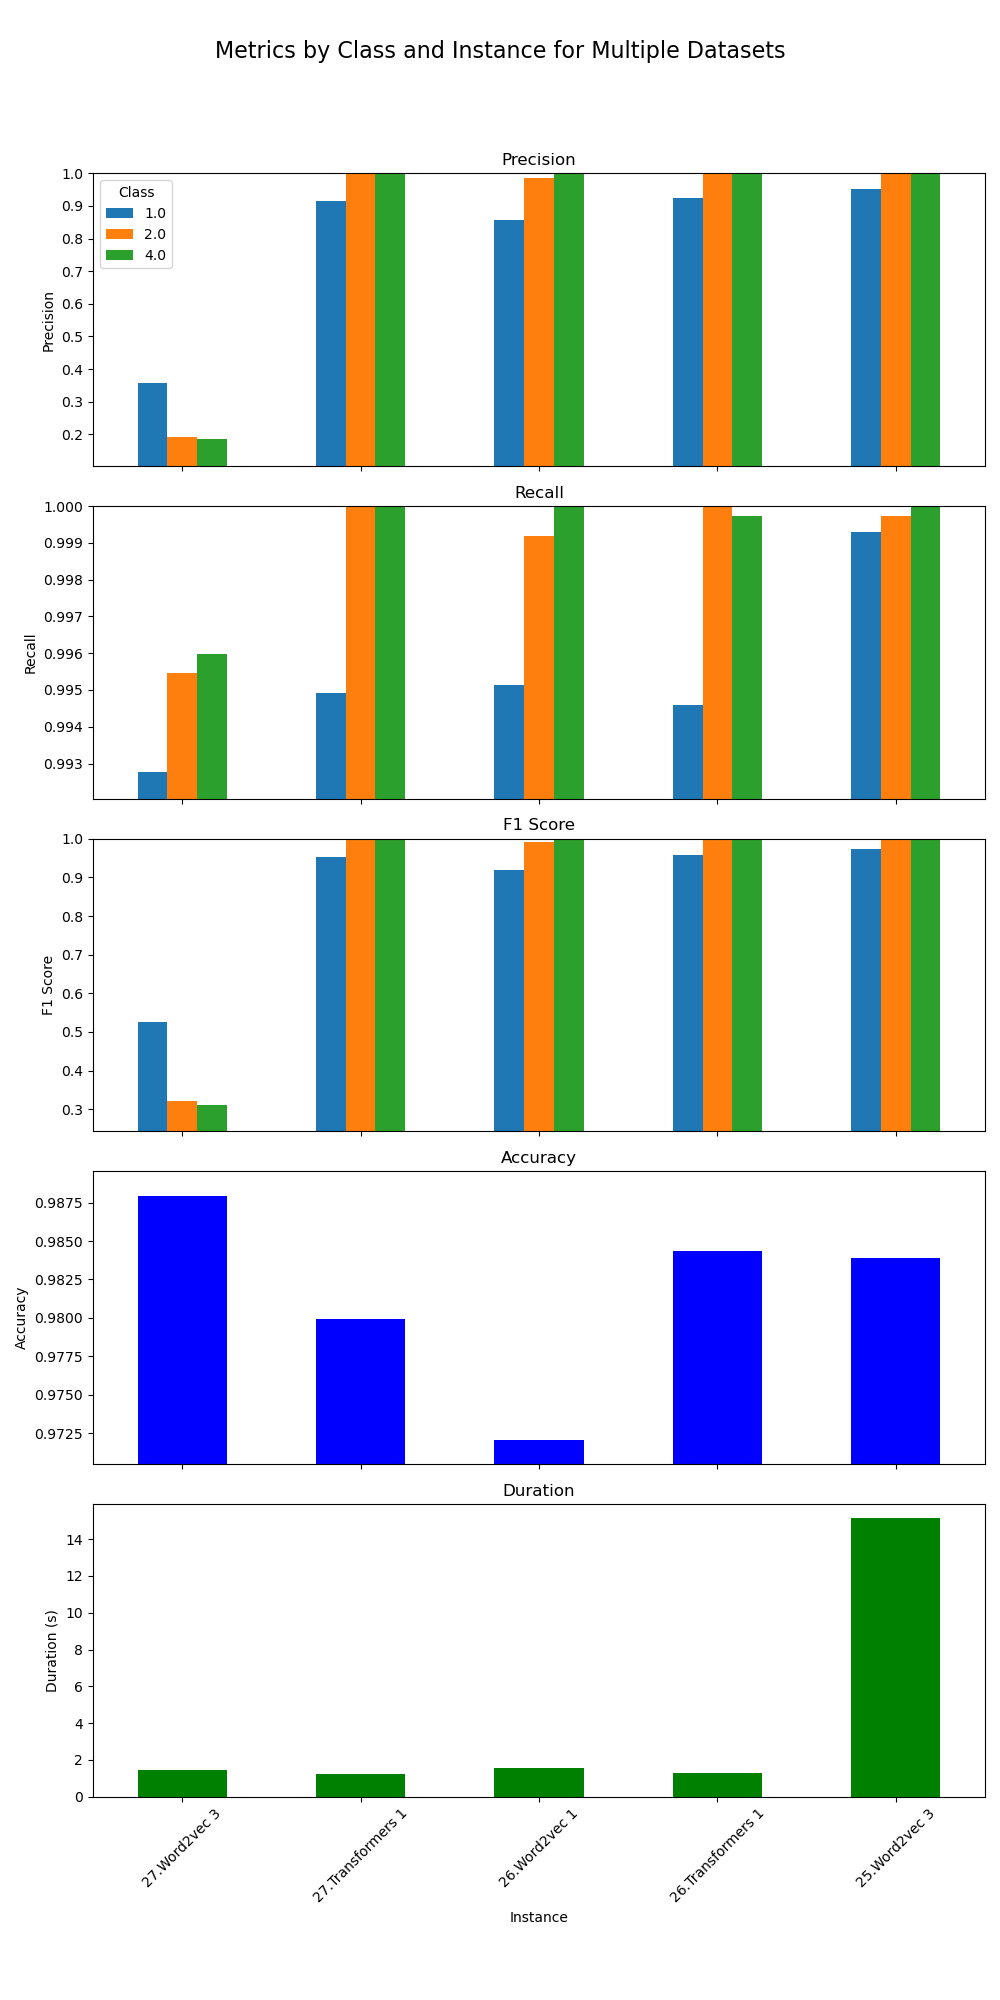
\includegraphics[width=0.6\textwidth]{img/annexes/Best Accuracy (by instances).png}
    \caption{Metrics for the best instances (accuracy)}
    \label{fig:results:best_accuracy_instances}
\end{figure}

\paragraph{}The two top-performing instances, both utilizing chunk\_start\_bytes\_embedding, achieved remarkable accuracy scores of 99.90\% with the chunk size filter~\ref{tab:21_single_instance_classifiers_results} and 99.84\% without the filter~\ref{tab:20_single_instance_classifiers_results}. Following closely was chunk\_semantic\_embedding with the chunk size filter, securing an accuracy of 99.70\%~\ref{tab:9_single_instance_classifiers_results}. Notably, the first deep learning model to make an appearance in the ranking was a Word2Vec model, which, with both entropy and chunk size filters applied, attained an accuracy of 98.79\%, placing it sixth overall~\ref{tab:27_word2vec_3_classifiers_results}.

\paragraph{}When focusing on recall for label 1, the best instance was chunk\_start\_bytes\_embedding without any filter, achieving a perfect recall of 100\%~\ref{tab:20_single_instance_classifiers_results}, as shown in Figure \ref{fig:results:best_label_1_recall_instances}. The second-best was again chunk\_start\_bytes\_embedding, this time with both entropy and chunk size filters, achieving a recall of 99.99553\%~\ref{tab:23_single_instance_classifiers_results}. The first deep learning model, a Word2Vec instance with both filters, ranked third with a recall of 99.95\%.

\begin{figure}[ht]
    \centering
    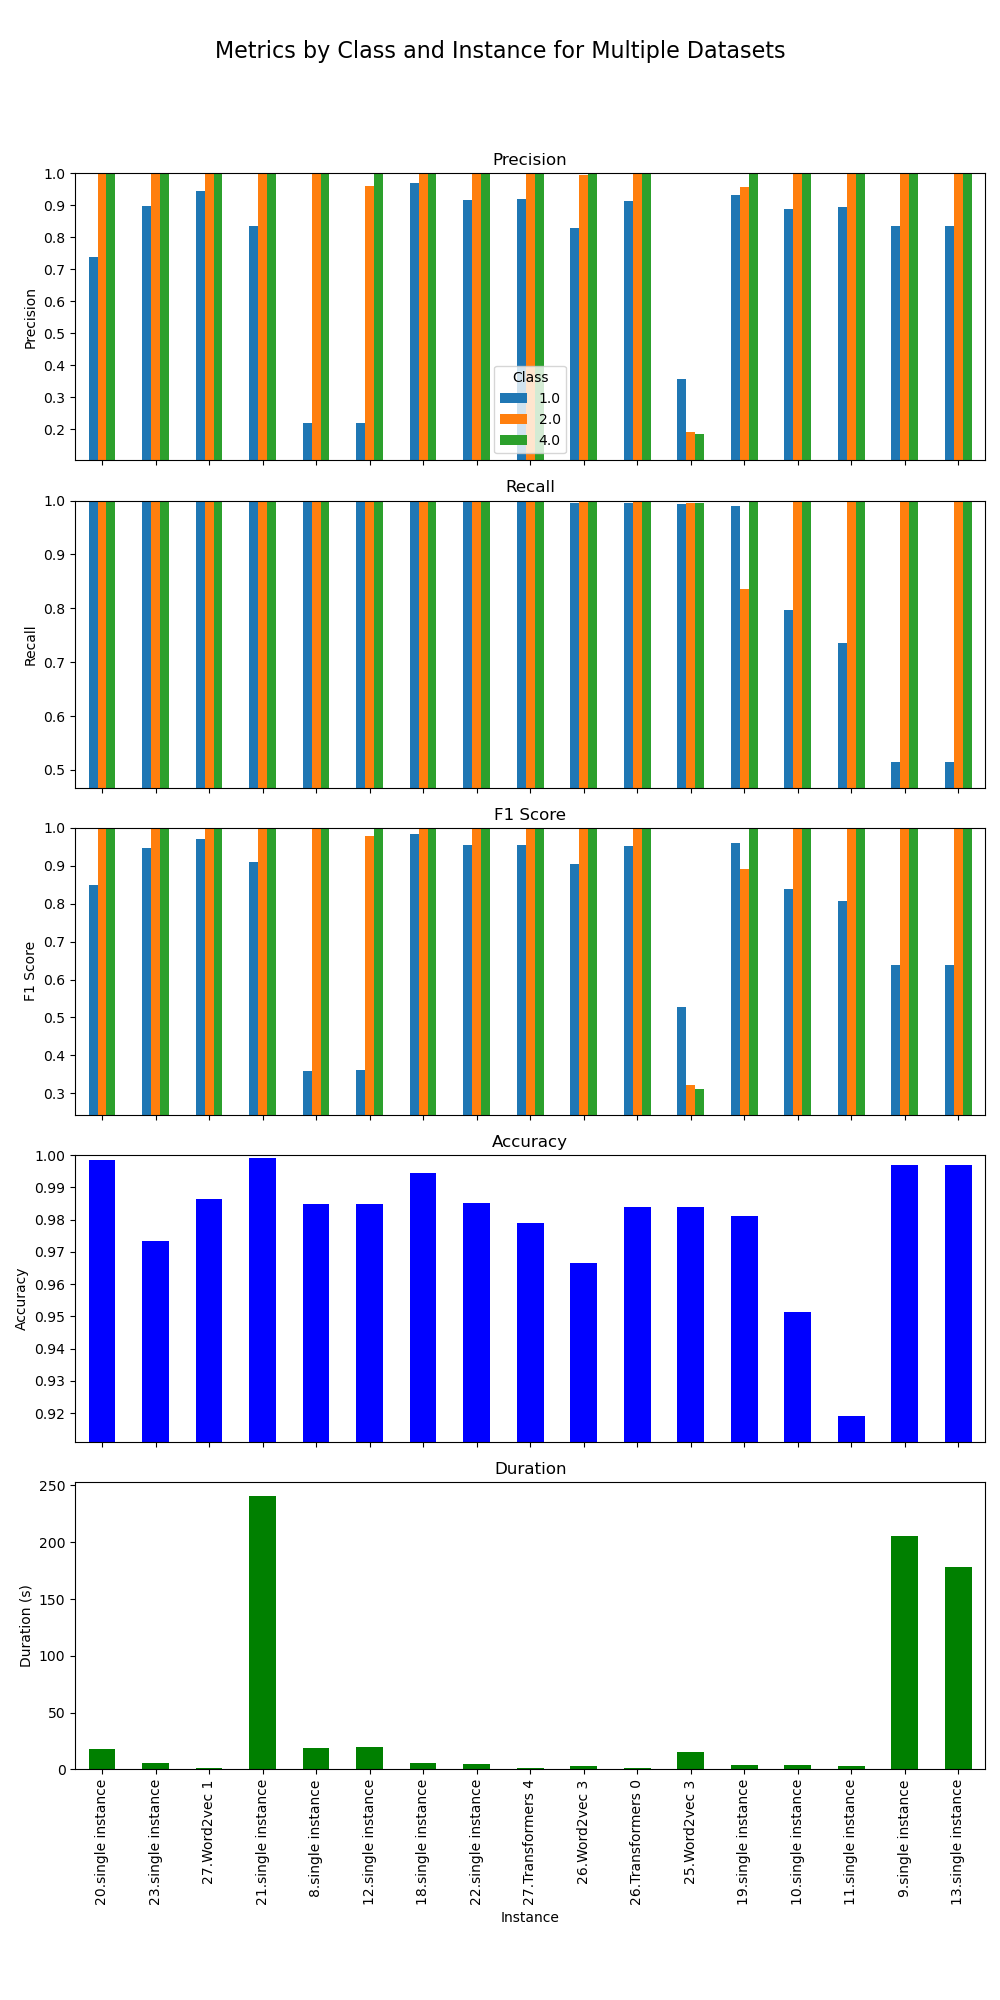
\includegraphics[width=0.6\textwidth]{img/annexes/Best 1.0 Recall (by instances).png}
    \caption{Metrics for the best instances (Label 1 recall)}
    \label{fig:results:best_label_1_recall_instances}
\end{figure}

\paragraph{}As for precision on label 1, the highest achievement was recorded by chunk\_statistic\_embedding with the entropy filter, which reached a precision of 96.86\%~\ref{tab:18_single_instance_classifiers_results}, as illustrated in Figure \ref{fig:results:best_label_1_precision_instances}. The second-highest precision came from a Word2Vec deep learning model with both entropy and chunk size filters, scoring 95.19\%.

\begin{figure}[ht]
    \centering
    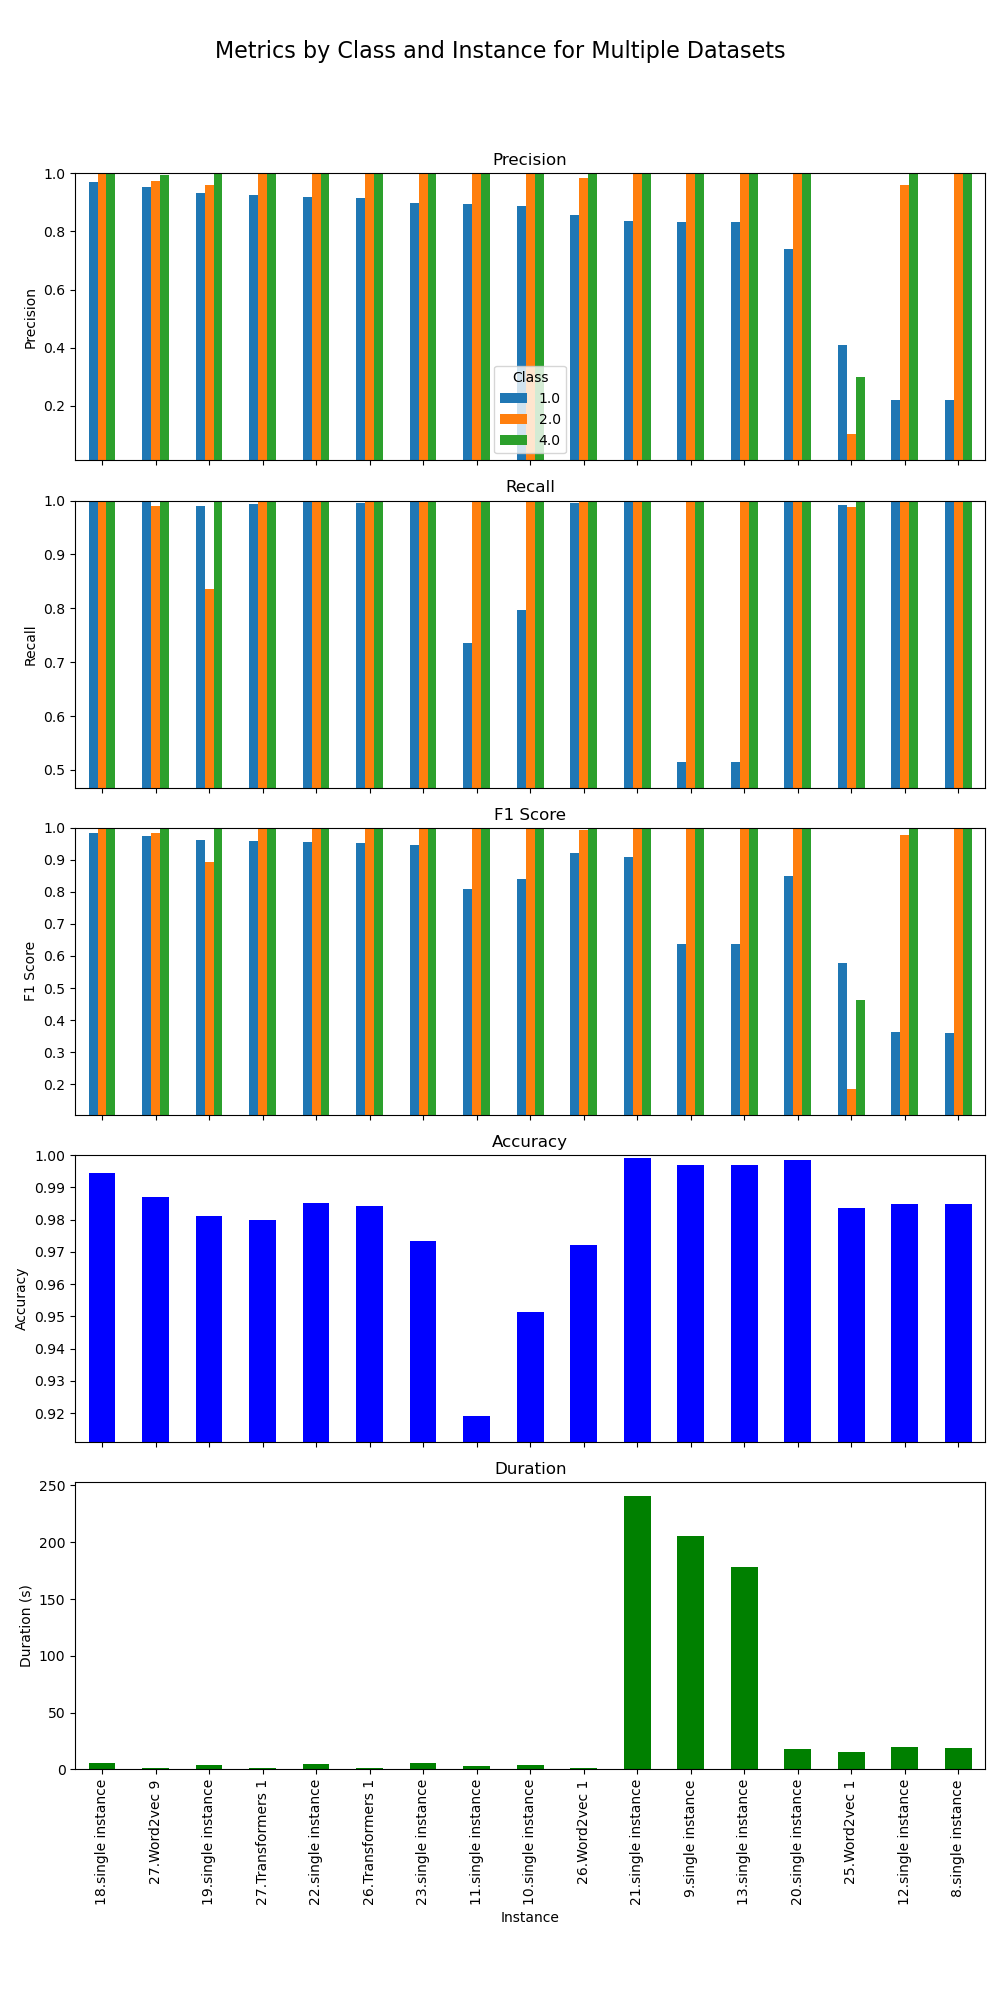
\includegraphics[width=0.6\textwidth]{img/annexes/Best 1.0 Precision (by instances).png}
    \caption{Metrics for the best instances (Label 1 precision)}
    \label{fig:results:best_label_1_precision_instances}
\end{figure}


\chapter{Discussion}\label{chap:discussion}


Discuss the results. What is the outcome of your experimetns?
\chapter{Conclusion}\label{chap:conclusion}

\paragraph{}In conclusion, this Master's thesis has provided a comprehensive survey of various embedding techniques for the classification of SSH keys in OpenSSH memory dumps. The study has uncovered that simple embedding techniques, such as the trim method and statistical approaches, yield highly effective results when applied to this specific dataset. Additionally, NLP techniques like Word2Vec and Transformers have shown promising outcomes, although they require further refinement through hyperparameter tuning to reach their full potential.

\paragraph{}While coherence testing has not been conclusively demonstrated, the classification results have been exceptionally positive, indicating the practical value of the research. However, there remains a substantial scope for future work. This includes measuring the time efficiency of the embedding processes, extensive hyperparameter optimization, exploration of additional NLP techniques, and more rigorous coherence testing. These areas present exciting opportunities for further research and development in the field of digital forensics and cybersecurity.

\chapter{Ressources}\label{chap:ressources}

\paragraph{}In the resources chapter of this thesis, we meticulously detail the various materials and tools that have been utilized throughout the course of the research. 

\section{hardware}
\paragraph{}My primary workstation is an \textit{Aspire 5} laptop, equipped with:
\begin{itemize}
    \item \textbf{CPU:} 11th Gen Intel i5-1135G7 (8) @ 4.200GHz 
    \item \textbf{GPU:} Intel TigerLake-LP GT2 [Iris Xe Graphics]
    \item \textbf{Memory:} 16GB
\end{itemize}
\paragraph{}However, this laptop, despite its decent specifications, proved inadequate for processing the entire dataset. Simple machine learning experiments using a Python script would have stretched over a week. Even when we transitioned to more optimized Rust programs, the processing time exceeded 10 hours. While we managed to run minor tasks and scripts on this laptop, the bulk of the experiments necessitated a more powerful server.

\paragraph{}Recognizing this need, we was granted access to a high-performance development server in the later stages of the thesis, around August 2023. The server, an \textit{AS-4124GS-TNR}, boasts the following specifications:
\begin{itemize}
    \item \textbf{CPU:} 2x AMD EPYC 7662 (256) @ 2.000GHz
    \item \textbf{GPU:} NVIDIA Geforce RTX 3090 Ti
    \item \textbf{RAM:} 512GB DDR4 3200MHz
\end{itemize}
\paragraph{}Operating on \textit{Ubuntu 20.04.6 LTS}, this server became the primary platform for the machine learning experiments, given its superior computational capabilities compared to the \textit{Aspire 5} laptop. This invaluable resource was generously provided by the Department of Computer Science at \textit{Universität Passau}, particularly under the guidance of the Chair of Data Science led by Prof. Dr. Michael Granitzer. I extend my sincere appreciation for their unwavering support.

\section{Code Repository}

\paragraph{}The code repository section of this thesis is dedicated to providing open access to all the data and code used throughout the research. Hosted on GitHub under the organization \textit{Passau Masterarbeit 2023}, the repositories are a testament to the commitment to transparency and collaborative development.

\paragraph{}The repository \textit{mem2graph}\footnote{\url{https://github.com/passau-masterarbeit-2023/mem2graph}} is particularly noteworthy as it contains the code for analyzing memory dumps and converting them into simple embeddings. This repository is a crucial resource for anyone looking to understand or replicate the memory dump analysis process.

\paragraph{}For those interested in the deep learning and machine learning aspects of the thesis, the repository \textit{phdtrack\_openssh\_memory\_embedding}\footnote{\url{https://github.com/passau-masterarbeit-2023/phdtrack_openssh_memory_embedding}} is invaluable. It not only includes the code for these processes but also houses the complete results of the experiments in the \texttt{results\_server\_full/} folder, providing a thorough record of the research findings.

\paragraph{}Lastly, the repository \textit{phdtrack\_server\_scripts}\footnote{\url{https://github.com/passau-masterarbeit-2023/phdtrack_server_scripts}} offers the scripts used to set up the environment on the server, ensuring that the computational setup can be replicated or adapted for future research endeavors.



%%%%%%%%%%%%%%%%%%%%%%%%%%%%%%%%%%%%%%%%%%%%%%%%%%%%%%%%%%%%%%%%%%%%%%%%%%%%%%%%%%%%%%%%%

% glossary and acronyms
\newpage
% \printglossary[type=\acronymtype, title=Acronymes]
% \printglossary[title=Glossaire]
\printglossary[type=\acronymtype]

\printglossary

% biblio
\newpage
\printbibliography[
    heading=bibintoc,
    category=cited,
    title={References}
]

% uncited references (bibliography)
% https://tex.stackexchange.com/questions/6967/how-to-split-bibliography-into-works-cited-and-works-not-cited
\printbibliography[
    notcategory=cited,
    heading=bibintoc,
    title={Additional bibliography},
]

\newpage
% -- Appendix (optional)
\begin{appendices}
    % !TeX spellcheck = en\_US
% !TeX encoding = UTF-8
\chapter{Models}
\section{Machin Learning Hyperparameters}
\subsection{Random Forest Classifier}

    \begin{table}[ht]
        \centering
        \caption{Default Parameters for Random Forest Classifier}
        \begin{tabular}{lc}
            \textbf{Parameter} & \textbf{Default Value} \\
            bootstrap & True \\
            ccp\_alpha & 0.0 \\
            class\_weight & None \\
            criterion & gini \\
            max\_depth & None \\
            max\_features & sqrt \\
            max\_leaf\_nodes & None \\
            max\_samples & None \\
            min\_impurity\_decrease & 0.0 \\
            min\_samples\_leaf & 1 \\
            min\_samples\_split & 2 \\
            min\_weight\_fraction\_leaf & 0.0 \\
            n\_estimators & 100 \\
            n\_jobs & -1 \\
            oob\_score & False \\
            random\_state & 42 \\
            verbose & 0 \\
            warm\_start & False \\
        \end{tabular}
    \end{table}

    \subsection{OPTICS Clustering}

    \begin{table}[ht]
        \centering
        \caption{Default Parameters for OPTICS Clustering}
        \begin{tabular}{lc}
            \textbf{Parameter} & \textbf{Default Value} \\
            algorithm & brute \\
            cluster\_method & xi \\
            leaf\_size & 30 \\
            max\_eps & inf \\
            memory & None \\
            metric & cosine \\
            metric\_params & None \\
            min\_cluster\_size & None \\
            n\_jobs & -1 \\
            p & 2 \\
            predecessor\_correction & True \\
            xi & 0.05 \\
        \end{tabular}
    \end{table}


    \paragraph{Note for OPTICS:}
    \begin{description}
        \item[min\_samples:] Calculated dynamically for each embedding.
        \item[eps:] Takes five distinct values: 0.01, 0.02, 0.03, 0.04, and 0.05.
    \end{description}

\section{Deep learning hyperparameters}
    \subsection{Transformers:}
        \begin{table}[ht]
            \centering
            \caption{Transformers Hyperparameters (Configurations 0–4)}
            \begin{tabular}{lccccc}
                & Config 0 & Config 1 & Config 2 & Config 3 & Config 4 \\
                word character size & 16 & 16 & 8 & 8 & 16 \\
                embedding dim & 8 & 16 & 8 & 16 & 8 \\
                transformer units & 2 & 2 & 2 & 2 & 4 \\
                num heads & 2 & 2 & 2 & 2 & 4 \\
                num transformer layers & 2 & 2 & 2 & 2 & 4 \\
                dropout rate & 0.1 & 0.1 & 0.1 & 0.1 & 0.3 \\
                activation & relu & relu & relu & relu & relu \\
            \end{tabular}
        \end{table}

        \begin{table}[ht]
            \centering
            \caption{Transformers Hyperparameters (Configurations 5–7)}
            \begin{tabular}{lccc}
                & Config 5 & Config 6 & Config 7 \\
                word character size & 16 & 8 & 8 \\
                embedding dim & 16 & 8 & 16 \\
                transformer units & 4 & 4 & 4 \\
                num heads & 4 & 4 & 4 \\
                num transformer layers & 4 & 4 & 4 \\
                dropout rate & 0.3 & 0.3 & 0.3 \\
                activation & relu & relu & relu \\
            \end{tabular}
        \end{table}


    \subsection{Word2Vec:}
        \begin{table}[ht]
            \centering
            \caption{Word2Vec Hyperparameters (Configurations 0–4)}
            \begin{tabular}{lccccc}
                & Config 0 & Config 1 & Config 2 & Config 3 & Config 4 \\
                output size & 8 & 8 & 8 & 8 & 16 \\
                window character size & 8 & 8 & 16 & 16 & 8 \\
                word character size & 2 & 4 & 2 & 4 & 2 \\
                min count & 1 & 1 & 1 & 1 & 1 \\
            \end{tabular}
        \end{table}

        \begin{table}[ht]
            \centering
            \caption{Word2Vec Hyperparameters (Configurations 5–9)}
            \begin{tabular}{lccccc}
                & Config 5 & Config 6 & Config 7 & Config 8 & Config 9 \\
                output size & 16 & 16 & 16 & 100 & 100 \\
                window character size & 8 & 16 & 16 & 8 & 8 \\
                word character size & 4 & 2 & 4 & 2 & 4 \\
                min count & 1 & 1 & 1 & 1 & 1 \\
            \end{tabular}
        \end{table}

        \begin{table}[ht]
            \centering
            \caption{Word2Vec Hyperparameters (Configurations 10–11)}
            \begin{tabular}{lcc}
                & Config 10 & Config 11 \\
                output size & 100 & 100 \\
                window character size & 16 & 16 \\
                word character size & 2 & 4 \\
                min count & 1 & 1 \\
            \end{tabular}
        \end{table}
    
    
\chapter{Dataset}

    \section{Dataset cleaning results}\label{sec:annexes:dataset_cleaning_results}
        \paragraph{}The empty folder for the training part of the dataset after cleaning are : 
        \begin{longtable}{|c|c|c|}
            \caption{List of empty Folders in the training subdataset Categorized by OpenSSH Parameters} \label{tab:annexes:dataset_cleaning_results:training_empty} \\
            \hline
            \textbf{Use Case} & \textbf{Version} & \textbf{Key Size} \\
            \hline
            \endfirsthead
            \multicolumn{3}{c}%
            {{\bfseries \tablename\ \thetable{} -- continued from previous page}} \\
            \hline
            \textbf{Use Case} & \textbf{Version} & \textbf{Key Size} \\
            \hline
            \endhead
            \hline
            \multicolumn{3}{|r|}{{Continued on next page}} \\
            \hline
            \endfoot
            \hline
            \endlastfoot
            % Data goes here, for example:
            port-forwarding & V\_8\_0\_P1 & 64 \\
            port-forwarding & V\_8\_0\_P1 & 32 \\
            port-forwarding & V\_7\_8\_P1 & 16 \\
            port-forwarding & V\_7\_8\_P1 & 64 \\
            port-forwarding & V\_7\_8\_P1 & 32 \\
            scp & V\_8\_0\_P1 & 64 \\
            scp & V\_8\_0\_P1 & 32 \\
            scp & V\_7\_8\_P1 & 64 \\
            scp & V\_7\_8\_P1 & 32 \\
            basic & V\_8\_7\_P1 & 16 \\
            basic & V\_8\_7\_P1 & 64 \\
            basic & V\_8\_7\_P1 & 32 \\
            basic & V\_8\_8\_P1 & 16 \\
            basic & V\_8\_8\_P1 & 64 \\
            basic & V\_8\_8\_P1 & 32 \\
            basic & V\_7\_0\_P1 & 16 \\
            basic & V\_7\_0\_P1 & 64 \\
            basic & V\_7\_0\_P1 & 32 \\
            basic & V\_6\_8\_P1 & 16 \\
            basic & V\_6\_8\_P1 & 64 \\
            basic & V\_6\_8\_P1 & 32 \\
            basic & V\_6\_2\_P1 & 16 \\
            basic & V\_6\_2\_P1 & 24 \\
            basic & V\_6\_2\_P1 & 32 \\
            basic & V\_6\_0\_P1 & 16 \\
            basic & V\_6\_0\_P1 & 24 \\
            basic & V\_6\_0\_P1 & 32 \\
            basic & V\_8\_1\_P1 & 16 \\
            basic & V\_8\_1\_P1 & 64 \\
            basic & V\_8\_1\_P1 & 32 \\
            basic & V\_6\_1\_P1 & 16 \\
            basic & V\_6\_1\_P1 & 24 \\
            basic & V\_6\_1\_P1 & 32 \\
            basic & V\_7\_2\_P1 & 16 \\
            basic & V\_7\_2\_P1 & 64 \\
            basic & V\_7\_2\_P1 & 32 \\
            basic & V\_8\_0\_P1 & 16 \\
            basic & V\_8\_0\_P1 & 64 \\
            basic & V\_8\_0\_P1 & 32 \\
            basic & V\_6\_3\_P1 & 16 \\
            basic & V\_6\_3\_P1 & 24 \\
            basic & V\_6\_3\_P1 & 32 \\
            basic & V\_6\_9\_P1 & 16 \\
            basic & V\_6\_9\_P1 & 64 \\
            basic & V\_6\_9\_P1 & 32 \\
            basic & V\_7\_1\_P1 & 16 \\
            basic & V\_7\_1\_P1 & 64 \\
            basic & V\_7\_1\_P1 & 32 \\
            basic & V\_7\_9\_P1 & 16 \\
            basic & V\_7\_9\_P1 & 64 \\
            basic & V\_7\_9\_P1 & 32 \\
            basic & V\_6\_7\_P1 & 16 \\
            basic & V\_6\_7\_P1 & 24 \\
            basic & V\_6\_7\_P1 & 32 \\
            basic & V\_7\_8\_P1 & 16 \\
            basic & V\_7\_8\_P1 & 64 \\
            basic & V\_7\_8\_P1 & 32 \\
            client & V\_8\_0\_P1 & 16 \\
            client & V\_8\_0\_P1 & 64 \\
            client & V\_8\_0\_P1 & 32 \\
            client & V\_7\_8\_P1 & 16 \\
            client & V\_7\_8\_P1 & 64 \\
            client & V\_7\_8\_P1 & 32 \\
            % ... repeat for all files
        \end{longtable}

        \paragraph{}The empty folder for the validation part of the dataset after cleaning are : 
        \begin{longtable}{|c|c|c|}
            \caption{List of empty Folders in the validation subdataset Categorized by OpenSSH Parameters} \label{tab:annexes:dataset_cleaning_results:validation_empty} \\
            \hline
            \textbf{Use Case} & \textbf{Version} & \textbf{Key Size} \\
            \hline
            \endfirsthead
            \multicolumn{3}{c}%
            {{\bfseries \tablename\ \thetable{} -- continued from previous page}} \\
            \hline
            \textbf{Use Case} & \textbf{Version} & \textbf{Key Size} \\
            \hline
            \endhead
            \hline
            \multicolumn{3}{|r|}{{Continued on next page}} \\
            \hline
            \endfoot
            \hline
            \endlastfoot
            % Data goes here, for example:
            port-forwarding & V\_8\_0\_P1 & 64 \\
            port-forwarding & V\_8\_0\_P1 & 32 \\
            port-forwarding & V\_7\_8\_P1 & 16 \\
            port-forwarding & V\_7\_8\_P1 & 64 \\
            port-forwarding & V\_7\_8\_P1 & 32 \\
            scp & V\_8\_0\_P1 & 64 \\
            scp & V\_8\_0\_P1 & 32 \\
            scp & V\_7\_8\_P1 & 64 \\
            scp & V\_7\_8\_P1 & 32 \\
            basic & V\_8\_7\_P1 & 16 \\
            basic & V\_8\_7\_P1 & 64 \\
            basic & V\_8\_7\_P1 & 32 \\
            basic & V\_8\_8\_P1 & 16 \\
            basic & V\_8\_8\_P1 & 64 \\
            basic & V\_8\_8\_P1 & 32 \\
            basic & V\_7\_0\_P1 & 16 \\
            basic & V\_7\_0\_P1 & 64 \\
            basic & V\_7\_0\_P1 & 32 \\
            basic & V\_6\_8\_P1 & 16 \\
            basic & V\_6\_8\_P1 & 64 \\
            basic & V\_6\_8\_P1 & 32 \\
            basic & V\_6\_2\_P1 & 16 \\
            basic & V\_6\_2\_P1 & 24 \\
            basic & V\_6\_2\_P1 & 32 \\
            basic & V\_6\_0\_P1 & 16 \\
            basic & V\_6\_0\_P1 & 24 \\
            basic & V\_6\_0\_P1 & 32 \\
            basic & V\_8\_1\_P1 & 16 \\
            basic & V\_8\_1\_P1 & 64 \\
            basic & V\_8\_1\_P1 & 32 \\
            basic & V\_6\_1\_P1 & 16 \\
            basic & V\_6\_1\_P1 & 24 \\
            basic & V\_6\_1\_P1 & 32 \\
            basic & V\_7\_2\_P1 & 16 \\
            basic & V\_7\_2\_P1 & 64 \\
            basic & V\_7\_2\_P1 & 32 \\
            basic & V\_8\_0\_P1 & 16 \\
            basic & V\_8\_0\_P1 & 64 \\
            basic & V\_8\_0\_P1 & 32 \\
            basic & V\_6\_3\_P1 & 16 \\
            basic & V\_6\_3\_P1 & 24 \\
            basic & V\_6\_3\_P1 & 32 \\
            basic & V\_6\_9\_P1 & 16 \\
            basic & V\_6\_9\_P1 & 64 \\
            basic & V\_6\_9\_P1 & 32 \\
            basic & V\_7\_1\_P1 & 16 \\
            basic & V\_7\_1\_P1 & 64 \\
            basic & V\_7\_1\_P1 & 32 \\
            basic & V\_7\_9\_P1 & 16 \\
            basic & V\_7\_9\_P1 & 64 \\
            basic & V\_7\_9\_P1 & 32 \\
            basic & V\_6\_7\_P1 & 16 \\
            basic & V\_6\_7\_P1 & 24 \\
            basic & V\_6\_7\_P1 & 32 \\
            basic & V\_7\_8\_P1 & 16 \\
            basic & V\_7\_8\_P1 & 64 \\
            basic & V\_7\_8\_P1 & 32 \\
            client & V\_8\_0\_P1 & 16 \\
            client & V\_8\_0\_P1 & 64 \\
            client & V\_8\_0\_P1 & 32 \\
            client & V\_7\_8\_P1 & 16 \\
            client & V\_7\_8\_P1 & 32 \\
            % ... repeat for all files
        \end{longtable}

        \paragraph{}The folders left for the training part of the dataset after cleaning are :
        \begin{longtable}{|c|c|c|}
            \caption{List of kept Folders in the Training subdataset Categorized by OpenSSH Parameters} \label{tab:annexes:dataset_cleaning_results:training_kept} \\
            \hline
            \textbf{Use Case} & \textbf{Version} & \textbf{Key Size} \\
            \hline
            \endfirsthead
            \multicolumn{3}{c}%
            {{\bfseries \tablename\ \thetable{} -- continued from previous page}} \\
            \hline
            \textbf{Use Case} & \textbf{Version} & \textbf{Key Size} \\
            \hline
            \endhead
            \hline
            \multicolumn{3}{|r|}{{Continued on next page}} \\
            \hline
            \endfoot
            \hline
            \endlastfoot
            port-forwarding & V\_8\_0\_P1 & 16 \\
            port-forwarding & V\_8\_0\_P1 & 24 \\
            port-forwarding & V\_7\_8\_P1 & 24 \\
            scp & V\_8\_0\_P1 & 16 \\
            scp & V\_8\_0\_P1 & 24 \\
            scp & V\_7\_8\_P1 & 16 \\
            scp & V\_7\_8\_P1 & 24 \\
            basic & V\_8\_0\_P1 & 24 \\
            basic & V\_7\_8\_P1 & 24 \\
            basic & V\_7\_1\_P1 & 24 \\
            basic & V\_7\_0\_P1 & 24 \\
            basic & V\_7\_9\_P1 & 24 \\
            basic & V\_8\_1\_P1 & 24 \\
            basic & V\_6\_9\_P1 & 24 \\
            basic & V\_8\_7\_P1 & 24 \\
            basic & V\_8\_8\_P1 & 24 \\
            basic & V\_6\_8\_P1 & 24 \\
            basic & V\_7\_2\_P1 & 24 \\
            client & V\_8\_0\_P1 & 24 \\
            client & V\_7\_8\_P1 & 24 \\

        \end{longtable}

        \paragraph{}The folders left for the validation part of the dataset after cleaning are :
        \begin{longtable}{|c|c|c|}
            \caption{List of kept Folders in the Validation subdataset Categorized by OpenSSH Parameters} \label{tab:annexes:dataset_cleaning_results:validation_kept} \\
            \hline
            \textbf{Use Case} & \textbf{Version} & \textbf{Key Size} \\
            \hline
            \endfirsthead
            \multicolumn{3}{c}%
            {{\bfseries \tablename\ \thetable{} -- continued from previous page}} \\
            \hline
            \textbf{Use Case} & \textbf{Version} & \textbf{Key Size} \\
            \hline
            \endhead
            \hline
            \multicolumn{3}{|r|}{{Continued on next page}} \\
            \hline
            \endfoot
            \hline
            \endlastfoot
            port-forwarding & V\_8\_0\_P1 & 16 \\
            port-forwarding & V\_8\_0\_P1 & 16 \\
            port-forwarding & V\_8\_0\_P1 & 24 \\
            port-forwarding & V\_7\_8\_P1 & 24 \\
            scp & V\_8\_0\_P1 & 16 \\
            scp & V\_8\_0\_P1 & 24 \\
            scp & V\_7\_8\_P1 & 16 \\
            scp & V\_7\_8\_P1 & 24 \\
            basic & V\_8\_0\_P1 & 24 \\
            basic & V\_7\_8\_P1 & 24 \\
            basic & V\_7\_1\_P1 & 24 \\
            basic & V\_7\_0\_P1 & 24 \\
            basic & V\_7\_9\_P1 & 24 \\
            basic & V\_8\_1\_P1 & 24 \\
            basic & V\_6\_9\_P1 & 24 \\
            basic & V\_8\_7\_P1 & 24 \\
            basic & V\_8\_8\_P1 & 24 \\
            basic & V\_6\_8\_P1 & 24 \\
            basic & V\_7\_2\_P1 & 24 \\
            client & V\_8\_0\_P1 & 24 \\
            client & V\_7\_8\_P1 & 24 \\
        \end{longtable}

        \paragraph{}The folders left for the performance test part of the dataset after cleaning are :
        \begin{longtable}{|c|c|}
            \caption{List of kept Folders in the Performance Test subdataset Categorized by OpenSSH Parameters} \label{tab:annexes:dataset_cleaning_results:performance_test_kept} \\
            \hline
            \textbf{Version} & \textbf{Key Size} \\
            \hline
            \endfirsthead
            \multicolumn{2}{c}%
            {{\bfseries \tablename\ \thetable{} -- continued from previous page}} \\
            \hline
            \textbf{Version} & \textbf{Key Size} \\
            \hline
            \endhead
            \hline
            \multicolumn{2}{|r|}{{Continued on next page}} \\
            \hline
            \endfoot
            \hline
            \endlastfoot
            V\_8\_0\_P1 & 32 \\
            V\_8\_0\_P1 & 16 \\
            V\_8\_0\_P1 & 24 \\
            V\_7\_8\_P1 & 32 \\
            V\_7\_8\_P1 & 16 \\
            V\_7\_8\_P1 & 24 \\
            V\_7\_1\_P1 & 32 \\
            V\_7\_1\_P1 & 16 \\
            V\_7\_1\_P1 & 24 \\
            V\_7\_9\_P1 & 32 \\
            V\_7\_9\_P1 & 16 \\
            V\_7\_9\_P1 & 24 \\
            V\_8\_1\_P1 & 32 \\
            V\_8\_1\_P1 & 16 \\
            V\_8\_1\_P1 & 24 \\

        \end{longtable}
    \chapter{Results}\label{chap:results}

\paragraph{}In this thesis, we undertake a thorough investigation of data embeddings and their effectiveness in predicting SSH keys within OpenSSH memory dumps. The results are methodically structured, starting with Data Preprocessing, where we lay a solid foundation by preparing the data for in-depth analysis. We proceed to evaluate Deep Learning Models, analyzing their architecture and limitations. This is succeeded by Feature Engineering, where we meticulously refine our data to improve model accuracy. Through Clustering analysis, we explore and identify underlying patterns within the data. Ultimately, we employ Classification techniques to accurately predict and categorize SSH keys, thus demonstrating the practical implications and utility of our research. 
    

\section{Data Preprocessing}

\paragraph{}In the data preprocessing stage, we meticulously calculated each embedding four times, which included the deep learning models. This repetition was to test all combinations of the two filters—entropy and chunk size. The purpose of this thorough approach was to discern the effectiveness of each filter, both individually and in combination, providing us with a clearer understanding of their impact on the data and the subsequent results. The different datasets used are detailed in Section \ref{sec:annexe:all_dataset}. The dataset codes are explained in the following table~\ref{tab:results:dataset_codes}:

\begin{table}[ht]
    \centering
    \begin{tabular}{|p{0.3\linewidth}|p{0.6\linewidth}|}
    \hline
    Dataset Code & Meaning \\ 
    \hline
    value\_node\_embedding & First graph embedding, with all nodes~\ref{sec:embedding:first_graph} \\ \hline
    chunk\_top\_vn\_semantic\_embedding & First graph embedding, keeping only the first block of each chunk~\ref{sec:embedding:first_graph_only_first_block} \\ \hline
    chunk\_semantic\_embedding & Second graph embedding~\ref{sec:embedding:updated_graph} \\ \hline
    chunk\_statistic\_embedding & Statistical embedding~\ref{sec:embedding:statistical} \\ \hline
    chunk\_start\_bytes\_embedding & Start bytes embedding~\ref{sec:embedding:trim_method} \\ \hline
    chunk\_extraction & Raw byte extraction with filters, to be fed into the deep learning model\\ \hline
    \end{tabular}
    \caption{Meanings of Dataset Codes}
    \label{tab:results:dataset_codes}
\end{table}


\section{Deep Learning Models}

\paragraph{}The exploration of hyperparameters is documented in Section \ref{sec:annexes:deep_learning_hyperparameters}. During our experiments, we encountered instances where some models either ran out of memory, as noted in Sections \ref{sec:annexe:out_of_memory_instances_classifications} and \ref{sec:annexe:out_of_memory_instances_clustering}, or experienced timeouts, detailed in Section \ref{sec:annexe:timeout_instances}. Consequently, our discussion will be confined to the results yielded by the models that successfully completed their runs.

\paragraph{}Within the cohort of operational deep learning models, we endeavored to identify the most proficient instance for each algorithm, whether it was Transformers or Word2Vec. However, we encountered a scarcity of successful instances, which impeded our ability to conclusively determine the optimal hyperparameters or to fully understand their impact on the classification metrics. It was observed that instances with a larger word size and a reduced embedding dimension were more likely to succeed, presumably due to the decreased computational load they required.

\section{Feature Engineering}
\paragraph{}During our feature engineering phase, we encountered a challenge that led to the elimination of certain embeddings. This was due to the invariance observed in the columns, an issue that is elaborated upon in Section \ref{sec:annexe:feature_engineering_fails}. The specific embedding that was rendered ineffective and subsequently removed was the semantic embedding of the first graph, as discussed in Section \ref{sec:embedding:graph_embedding}. This elimination was necessary regardless of whether the filter on the first block of each chunk was applied. The primary shortcoming of this embedding was its inability to generate a sufficient number of ancestors to provide useful information. This inadequacy arose because only a minor segment of the value nodes were being pointed to by pointers, which significantly limited the utility of the embedding. In contrast, the second graph managed to compress the information effectively, thereby validating the semantic embedding by conveying more meaningful data for each node.

\paragraph{}The instances that successfully passed the feature engineering stage are meticulously recorded in Section \ref{sec:annexe:feature_engineering_results}. Here, the eight most significant columns are identified.

\section{Clustering}
\paragraph{}In the clustering phase of our analysis, we categorized the data into distinct groups: label 1 for SSH keys, label 2 for "ssh\_struct", label 4 for "session\_state\_struct", and label 0 for the remainder. The detailed outcomes of this clustering are presented in appendix \ref{sec:annexe:clustering_results}. Our examination revealed that the majority of clusters did not exhibit discernible patterns. However, certain datasets, such as those represented by chunk\_start\_bytes\_embedding (23) in Table \ref{tab:23_single_instance_clustering_results} and chunk\_statistic\_embedding (18) in Table \ref{tab:18_single_instance_clustering_results}, maintained a ratio of labels similar to that of the original dataset.


\paragraph{}Interestingly, the clusters derived from deep learning models typically displayed an even distribution of labels, with approximately one quarter of the data falling into each category. An exception to this trend was observed in the Word2Vec 3 Clustering Results on dataset 25 (with chunk size filter), as shown in Table \ref{tab:25_word2vec_3_clustering_results}, which consisted of three clusters with seemingly random label proportions.

\paragraph{}The results from the clustering analysis were not entirely definitive, indicating that there is substantial room for improvement in the methodology. Future efforts in this area would benefit from a more refined approach to enhance the clarity and significance of the clustering outcomes.

\section{Classification}

\paragraph{}The classification results of our study, detailed in appendix \ref{sec:annexe:classification_results}, yielded highly promising results. The performance of various instances, particularly in terms of accuracy, is depicted in the graphical representation found in Figure \ref{fig:results:best_accuracy_instances}, which ranks the instances from best to worst.

\begin{figure}[ht]
    \centering
    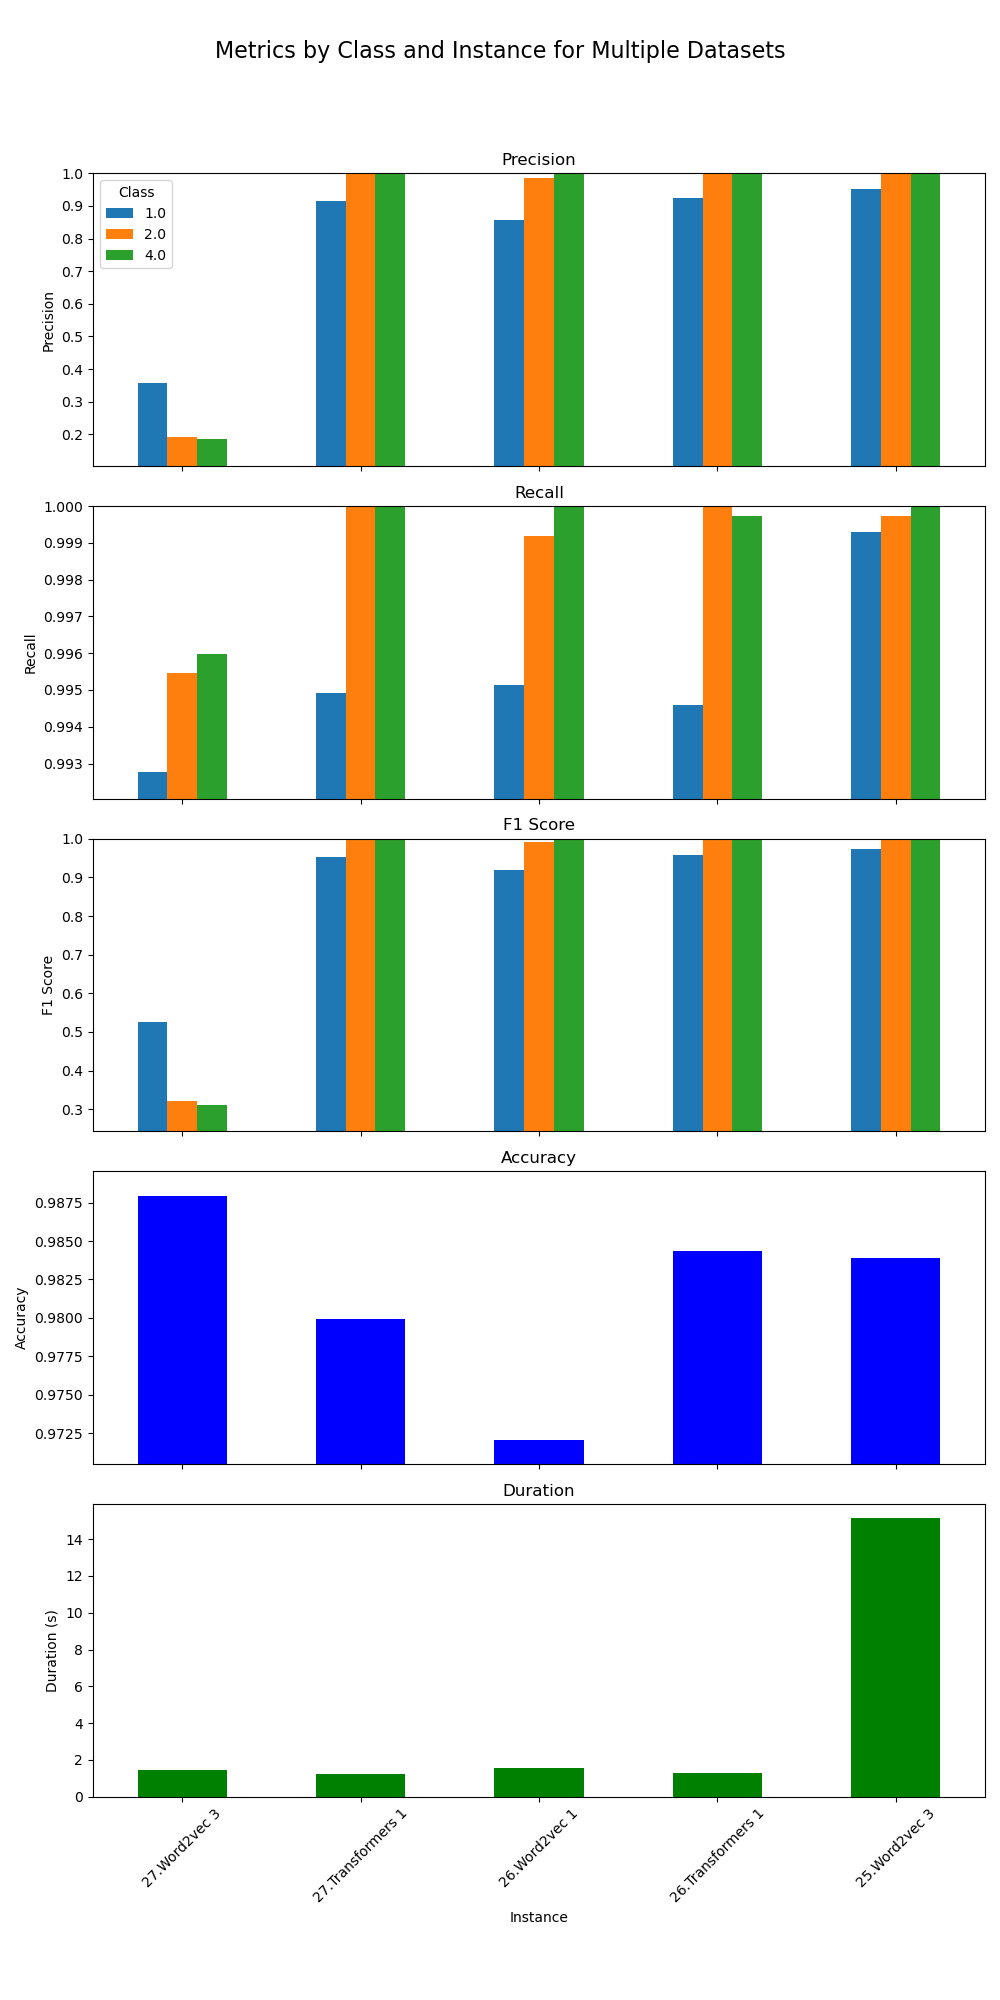
\includegraphics[width=0.6\textwidth]{img/annexes/Best Accuracy (by instances).png}
    \caption{Metrics for the best instances (accuracy)}
    \label{fig:results:best_accuracy_instances}
\end{figure}

\paragraph{}The two top-performing instances, both utilizing chunk\_start\_bytes\_embedding, achieved remarkable accuracy scores of 99.90\% with the chunk size filter~\ref{tab:21_single_instance_classifiers_results} and 99.84\% without the filter~\ref{tab:20_single_instance_classifiers_results}. Following closely was chunk\_semantic\_embedding with the chunk size filter, securing an accuracy of 99.70\%~\ref{tab:9_single_instance_classifiers_results}. Notably, the first deep learning model to make an appearance in the ranking was a Word2Vec model, which, with both entropy and chunk size filters applied, attained an accuracy of 98.79\%, placing it sixth overall~\ref{tab:27_word2vec_3_classifiers_results}.

\paragraph{}When focusing on recall for label 1, the best instance was chunk\_start\_bytes\_embedding without any filter, achieving a perfect recall of 100\%~\ref{tab:20_single_instance_classifiers_results}, as shown in Figure \ref{fig:results:best_label_1_recall_instances}. The second-best was again chunk\_start\_bytes\_embedding, this time with both entropy and chunk size filters, achieving a recall of 99.99553\%~\ref{tab:23_single_instance_classifiers_results}. The first deep learning model, a Word2Vec instance with both filters, ranked third with a recall of 99.95\%.

\begin{figure}[ht]
    \centering
    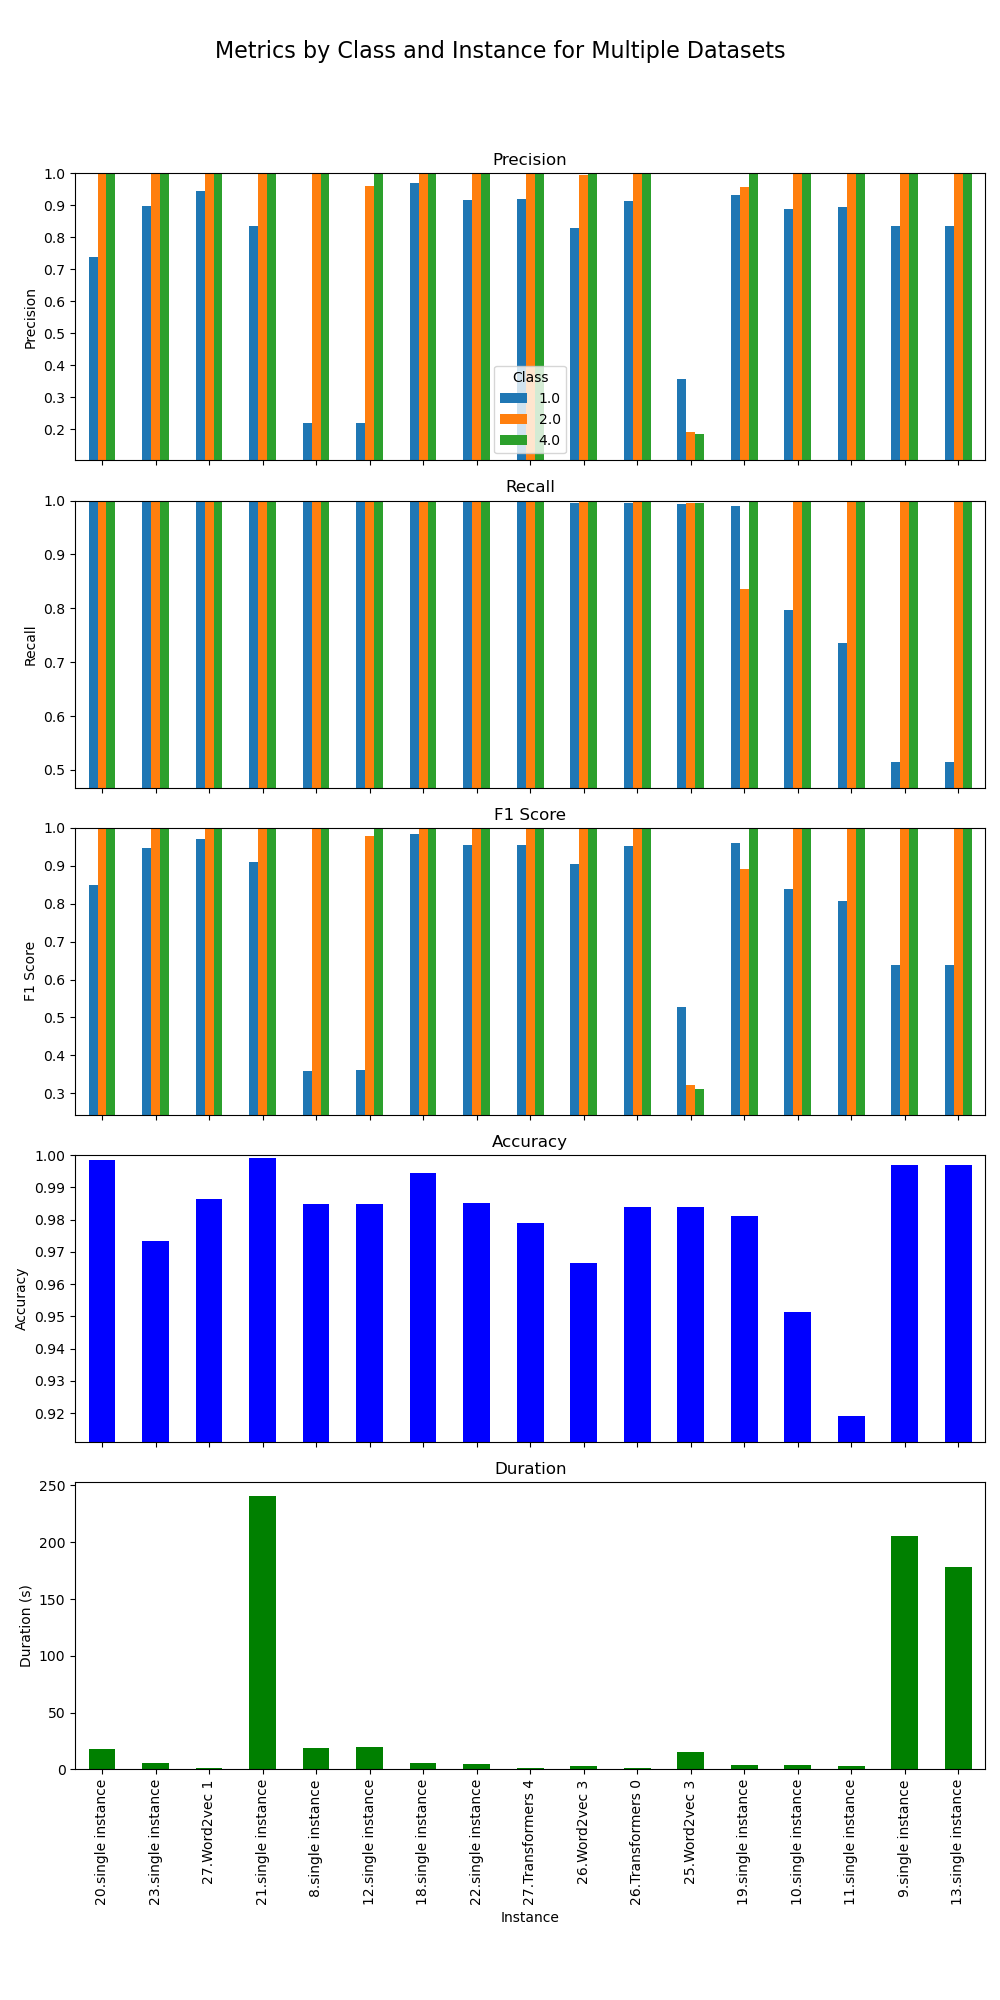
\includegraphics[width=0.6\textwidth]{img/annexes/Best 1.0 Recall (by instances).png}
    \caption{Metrics for the best instances (Label 1 recall)}
    \label{fig:results:best_label_1_recall_instances}
\end{figure}

\paragraph{}As for precision on label 1, the highest achievement was recorded by chunk\_statistic\_embedding with the entropy filter, which reached a precision of 96.86\%~\ref{tab:18_single_instance_classifiers_results}, as illustrated in Figure \ref{fig:results:best_label_1_precision_instances}. The second-highest precision came from a Word2Vec deep learning model with both entropy and chunk size filters, scoring 95.19\%.

\begin{figure}[ht]
    \centering
    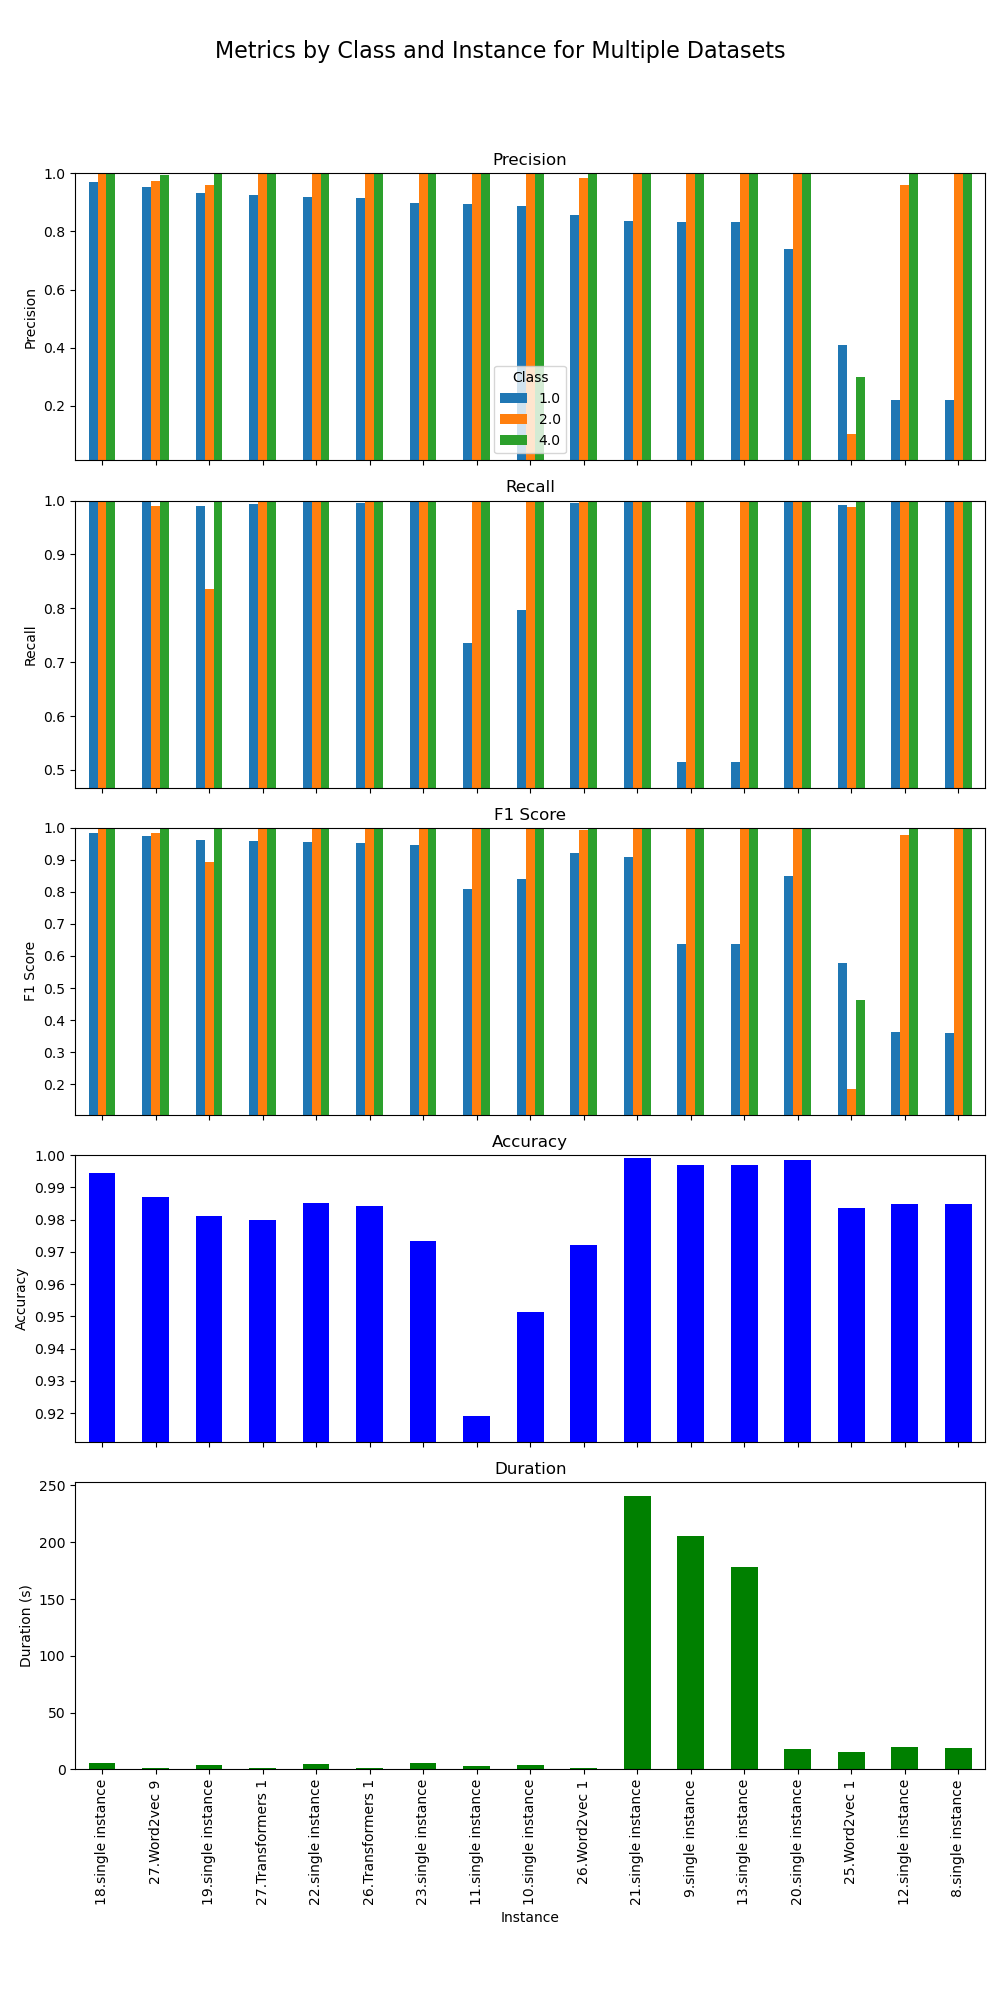
\includegraphics[width=0.6\textwidth]{img/annexes/Best 1.0 Precision (by instances).png}
    \caption{Metrics for the best instances (Label 1 precision)}
    \label{fig:results:best_label_1_precision_instances}
\end{figure}


\end{appendices}

% -- Eidesstattliche Erklrung (= Affadavit)
% !TeX spellcheck = de_DE
% !TeX encoding = UTF-8

\section*{Eidesstattliche Erkl\"arung}

	Hiermit versichere ich, dass ich diese Masterarbreit selbstst\"andig und ohne Benutzung anderer als der angegebenen Quellen und Hilfsmittel angefertigt habe und alle Ausf\"uhrungen, die w\"ortlich oder sinngem\"a\ss{} übernommen wurden, als solche gekennzeichnet sind, sowie, dass ich die Masterarbreit ~in gleicher oder \"ahnlicher Form noch keiner anderen Pr\"ufungsbeh\"orde vorgelegt habe.

	\vspace{3cm}

	Passau, \today

	\vspace{2cm}

	\parbox{8cm}{
		\hrule \strut \theauthor
	}



\restoregeometry
\end{document}